%%%%%%%%%%%%%%%%%%%%%%%%%%%%%%%%%%%%%%%%
% PDF compatibility code. 

\makeatletter
\newif\ifpdflatex@
\ifx\pdftexversion\@undefined
\pdflatex@false
%\message{Not using pdf}
\else
\pdflatex@true
%\message{Using pdf}
\fi

\newcommand{\latexorpdf}[2]{
  \ifpdflatex@ #2
  \else #1
  \fi
}

#ifdef A4Format
\newcommand{\pformat}{a4paper}
#endif A4Format
#ifdef LetterFormat
\newcommand{\pformat}{letterpaper}
#endif LetterFormat
\makeatother

\newcommand{\vdmtools}{\textbf{VDMTools}$^{\mathbf{{\textregistered}}}$}


%%%%%%%%%%%%%%%%%%%%%%%%%%%%%%%%%%%%%%%%

\latexorpdf{
\documentclass[\pformat,12pt,twoside]{article}
}{
% pdftex option is used by graphic[sx],hyperref,toolbox.sty
\documentclass[\pformat,pdftex,12pt]{article}
}

\usepackage{color}
\usepackage{colortbl}
\usepackage{alltt}

\newcolumntype{G}{>{\columncolor[gray]{0.8}}p{.98\textwidth}}
\newenvironment{VDMgray}%
{\begin{tabular}{|G|}\hline\small\begin{alltt}}%
{\end{alltt}\normalsize\\
 \hline\end{tabular}}

\usepackage{times}
\usepackage{graphicx}
\usepackage{longtable,multirow}
\latexorpdf{
\usepackage[plainpages=true,colorlinks,linkcolor=black,citecolor=black,%
            pagecolor=black, urlcolor=black]{hyperref}
}{
\usepackage[plainpages=true,colorlinks]{hyperref}
}

\usepackage{toolbox}
\usepackage{longtable}
%\usepackage{ifthen}
% plainpages=false: avoid warning
%   destination with the same identifier already exists
%   but it do not seem to work a the first pages

\usepackage{vpp}





\newcommand{\vdmtoolsver}{V6.8.5}

\makeatletter
% ------------- TOC manipulation ------------
\def\docglbldepth{1}

%\setcounter{secnumdepth}{\docglbldepth}
\setcounter{tocdepth}{2}

%\def\@pnumwidth{3.0em}

% more space for for >10 subsections
%\def\l@section{\@dottedtocline{1}{1.5em}{3.1em}}

%\def\l@subsection{\@dottedtocline{2}{1.5em}{2.8em}}

%\def\l@subsubsection{\@dottedtocline{3}{4.3em}{3.6em}}
%\def\l@paragraph{\@dottedtocline{4}{7.9em}{4.1em}}
%\def\l@subparagraph{\@dottedtocline{5}{10em}{5em}}
\makeatother

\definecolor{color16}{rgb}{0.53,0.53,0.53}

\begin{document}

\vdmtoolsmanual{A ``Cash-point'' Service Example}
       {\vdmtoolsver}
       {2005}
       {VDM-SL and VDM++}

\section{Introduction}


This document gives an overview of how
\vdmtools\ can be used in
different stages of the system/software development process. It can be
seen as an extension of the general guidelines provided in
\cite{Guidelines}. The
application example is a ``Cash-point'' service system. The document
first provides an overview of the informal requirements from the
system and then it proceeds with how we at IFAD envisage that a
problem such as this one should be attacked using
\vdmtools\ \cite{Mukherjee95a,Elmstrom&94}. VDM is a
model-oriented formal method for which many papers and books have been
published \cite{Jones90a,Fitzgerald&98b}. VDM-SL is the specification
language for VDM \cite{ISOVDM96} and VDM++ is an object-oriented
extension of that \cite{LangManPP}.
In the process we will also report on the kinds of discrepencies we found
during the development. We go 
through the following three steps:


\begin{description}
\item[Analysis] First, we develop an abstract model in VDM-SL in 
order to clarify and analyse requirements. This model is validated 
using a testing approach, e.g. allowing an imaginary client to 
test the model using a simple graphical front-end. The front-end 
is developed in Java and communicates with \vdmtools\  
via its Corba compliant API \cite{OMG&96,APIMan}. This illustrates the use of the 
VDM technology for both precise modelling and rapid prototyping 
in analysis.
\item[Design] Next, an OO version is developed in VDM++ incorporating
additional wishes from the client. For example, this model supports
the use of more than one till. The same front-end as before is used to
test this model together with the client. In particular, this step
demonstrates the interface to Rational Rose \cite{Rose&00} of
\vdmtools, combining the complementary benefits of visual modelling
using UML and precise modelling and validation using VDM++. This VDM++
design model was also systematically tested using \vdmtools\ and the
test coverage of the test suite is illustrated in
Appendix~\ref{app:VDMPP}.  Then a concurrent VDM++ design model is
developed. In this version an additional aspect is modelled: potential
communication failure between a till and the central resource. This
version of the VDM++ model is also connected to the same GUI as used
in the first design phase.
\item[Implementation] Finally, the concurrent VDM++ model is
implemented using the Java programming language \cite{Gosling&00} using the automatic code
generator of \vdmtools\ \cite{CGJavaManPP}.  This both ensures
consistency between the model and the implementation and dramatically
reduces the length of the coding phase. This version is again
connected to the same GUI as used in the design phases.
\end{description}

The purpose of our models is to analyse the main functional aspects 
of the system, including security aspects related to misuse of 
cards. For example, the models treat the daily limit policy, 
the validation of PIN codes, limits on PIN code attacks, and 
reports of illegal (e.g. stolen) cards. However, we abstract 
away from, for example, the choice of concrete databases, communication 
protocols and encoding of PIN codes. 

We believe that 
\vdmtools\ 
 is particularly strong in the 
following areas:
\begin{itemize}
\item 
Precise model of requirements with several pre-conditions and 
invariants
\item
Early validation of models
\item
Rapid prototyping where a client provides feedback on a model
\item
Automatic code generation of a concurrent system in Java
\item
Integration with leading tools in software development, including 
Word, Rose and JDK (Java)
\end{itemize}

This document is structured such that it starts off with an informal
description of the ``cash-point'' service example used in
Section~\ref{sec:req}. This is followed by four sections providing an
overview of the four models (for analysis, design, concurrent design and
implementation) from Section~\ref{sec:VDMSL} to
Section~\ref{sec:javaimpl}. Concluding remarks about the different
models and the approach illustrated in this document is given in
Section~\ref{sec:conclude}. After a list of the references the
different models are presented in full in different Appendices (A to
C). Throughout this document basic knowledge about the VDM-SL
\cite{ISOVDM96,Fitzgerald&98b} and VDM++ \cite{LangManPP,Guidelines}
is assumed.

\section{The Informal requirement Description}\label{sec:req}

In this section we provide a description of the system as formulated
from a customer.

\begin{quote}
There are many tills which can access a central resource containing
the detailed records of customers' bank accounts. A till is used by
inserting a card and typing in a PIN (Personal Identification Number)
which is encoded by the till and compared with a code stored on the
card.

After successfully identifying themselves to the system, customers may
try to:

\begin{enumerate}
\item view the balance of their accounts
\item make a withdrawal of cash
\item ask for a statement of their account to be sent by post
\end{enumerate}

Information on accounts is held in a central database and may be
unavailable. In that case 1) above may not be possible. If the
database is available, any amount up to the total in the account may
be withdrawn, subject to a fixed daily limit on withdrawals. This
means that the amount withdrawn within the day must be stored on the
card.

``Illegal'' cards are kept by the till.

The solution should consider feasible implementation
architectures. These are likely to include a data line between each
till and the central database. For example, transactions at a till may
be recorded locally and sent in a queue down the line to the central
database.

\textbf{Concurrency, time constraints}

It should be possible to show that the solution allows concurrent access
to the database from two or more different tills. It is important that
once a user has initiated a transaction, the transaction is completed
at least eventually, and preferably within some real time constraint.

You should also consider how to handle concurrent attempts from two
card holders who are authorised to use the same account.

\textbf{Security, reliability}

Clearly, for this sort of application, it is important to minimise the
possibility of the use of stolen cards to gain access to an account,
and that implementations of the system are robust against various
hazards such as poor transmission between a till and the central
database. Any way the solution can address such issues will be
particularly welcome.
\end{quote}

\section{VDM-SL Model}\label{sec:VDMSL}

The purpose of our first model is to make a quick analysis of 
the main functional requirements, essentially ignoring concurrency 
issues. Thus, this model describes aspects of the central resource 
and only one till. Once the basic functionality is better understood 
we start to consider multiple tills.

The model is described in VDM-SL as a short, flat specification. 
This enables abstraction from design considerations and ensures 
maximum focus on high-level, precise and systematic analysis. 
The specification is written in a Word file (RTF) and documented 
using standard text-processing facilities. \vdmtools\  
reads such Word documents and extracts the VDM parts. It also 
provides a pretty-printer for RTF documents. The pretty-printed 
VDM-SL specification is included in Appendix A.


Our VDM-SL model covers the following aspects documented in the 
requirements:
\begin{itemize}
\item
Accounts cannot be overdrawn and have a negative balance. Ensured 
in the withdrawal operation and by using a natural number to 
model the balance of an account.
\item
The daily limit for an account cannot be exceeded. Ensured in 
the withdrawal operation and using an elegant invariant on the 
transactions of an account. \textbf{NB!} Since daily limits are related 
to accounts we see no need to store transactions on cards. This 
decision goes against the requirements, and would need to be 
clarified with the client.
\item
Cards are validated before they are used. Ensured in the validation 
operation and in several pre-conditions of operations.
\item
The till keeps cards that are illegal when they are validated. 
We assume that a set of illegal card ids is stored by the central 
resource.
\item
Main functions numbered as 1, 2, and 3 in the informal description in
Section~\ref{sec:req} above
are specified precisely. Pre-conditions ensure that they are 
used correctly, e.g. it is required that there is a legal card 
in the till before an operation is allowed. Legal cards must 
not be among illegal cards and must hold a valid account and 
card id. In addition the withdrawal operation is made safe as 
it checks the balance and daily limit conditions prior to performing 
a transaction.
\end{itemize}


Our VDM-SL model covers the following aspects which are not mentioned 
in the requirements:
\begin{itemize}
\item
A till can service only one card at a time. Ensured in the pre-condition 
of \texttt{\emph{InsertCard}}.
\item
Account ids must be unique. Ensured using a map type.
\item
Card ids must be unique across accounts. Ensured using an invariant 
and a map type.
\item
If a correct PIN code has been entered, it cannot be re-entered 
in the same session.
\item
A function has been added to return a card. This allows a user 
of a till to return a card during a session and to perform several 
transactions in one session.
\end{itemize}


\vdmtools\  supports the execution of VDM-SL 
models, where properties documented in invariants and pre-conditions 
are checked automatically during execution. This facility is 
used by the specifier to validate a model in an interactive or 
systematic way. Via the Corba compliant API of \vdmtools, 
it is also possible to execute models from other code, e.g. a 
graphical front-end. We made such a rapid prototype GUI in Java 
to allow a client to test the model. Our simple interface of 
the till is shown in Figure~\ref{fig:VDMSLscreen}.

Let us assume that our imaginary client accepts our first model 
except for one thing. After extensive testing using the graphical 
front-end the client finds out that it is possible to break the 
PIN code by repeated attempts. The client wants a limit on the 
number of tries per day. This is incorporated in the next model 
of the system. Thus the analysis has improved both our and the 
client's understanding of the requirements and what the client 
really wants.

\begin{figure}[htbp]
\begin{center}
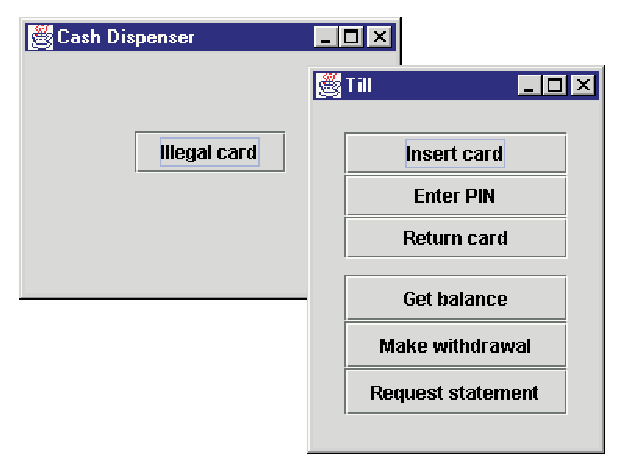
\includegraphics[width=.7\textwidth]{slscreen}
\caption{Prototype GUI for VDM-SL model.\label{fig:VDMSLscreen}}
\end{center}
\end{figure}

\section{VDM++ Model}\label{sec:VDMPP}


Our second model continues the development summarised above, 
but is more design-oriented. It presents an OO model in VDM++, 
which incorporates multiple tills and the additional requirement 
from the client on the limit on the number of failures to enter 
a correct PIN code.

\noindent
\begin{figure}[tb]
\begin{center}
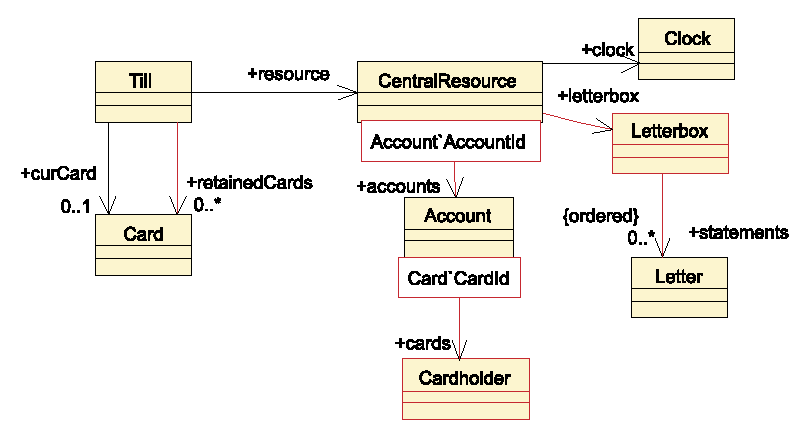
\includegraphics[width=.9\textwidth]{classoverview2}
\caption{First overall UML class diagram.\label{fig:VDM++overview}}
\end{center}
\end{figure}

As the VDM++ model does not add much new functionality to the 
system, we shall not repeat the points summarised above. Instead 
let us say a few words about the development of the VDM++ model. 
We start by identifying classes using a traditional approach. 
The state of the VDM-SL model is split into a \texttt{\emph{CentralResource}} 
class and a \texttt{\emph{Till}} class. Most other classes correspond to records 
in the VDM-SL model. It is decided to keep Transaction as a record 
in the OO model, as it is merely a container class without any 
obvious functionality relative to the current focus of our model. 
Once we have decided on which classes to include in our model, 
we sketch the classes in Rational Rose and establish relations 
between them (see Figure~\ref{fig:VDM++overview}). In order to focus more on 
account statements sent to cardholders, there are additional 
classes for \texttt{\emph{Letter}}s and a \texttt{\emph{Letterbox}}. The \texttt{\emph{Clock}} class keeps the 
date. In \cite{Guidelines} more discussion is made about the decision of
modelling via types or classes.

Using \vdmtools\  this UML model is then automatically 
translated into VDM++ resulting in a number of skeleton classes. 
Additional details are added, such as attributes of classes and 
signatures of operations. 
At any time the UML model can be updated according to the changes 
in the VDM++ model, and vice versa, using the Rose-VDM++ Link 
of \vdmtools\  which supports round-trip engineering 
in this sense. The complete UML class diagram of the system is shown 
in Figure~\ref{fig:VDM++full}. The corresponding, detailed VDM++ model is presented in 
Appendix B. The UML model gives a good overview of the system, 
but lacks the detailed knowledge found in analysis. The VDM++ 
model is precise and provides a much stronger basis for implementation. 
In this way the two models, or the two views of the same model, 
complement each other.

Another benefit of the VDM++ model is that it is more design-oriented 
than the VDM-SL model, yet all requirements are described precisely 
in the model. Therefore the VDM++ model is easier to implement 
and makes the early VDM-SL model obsolete in the later stages 
of development.

\noindent
\begin{figure}[tb]
\begin{center}
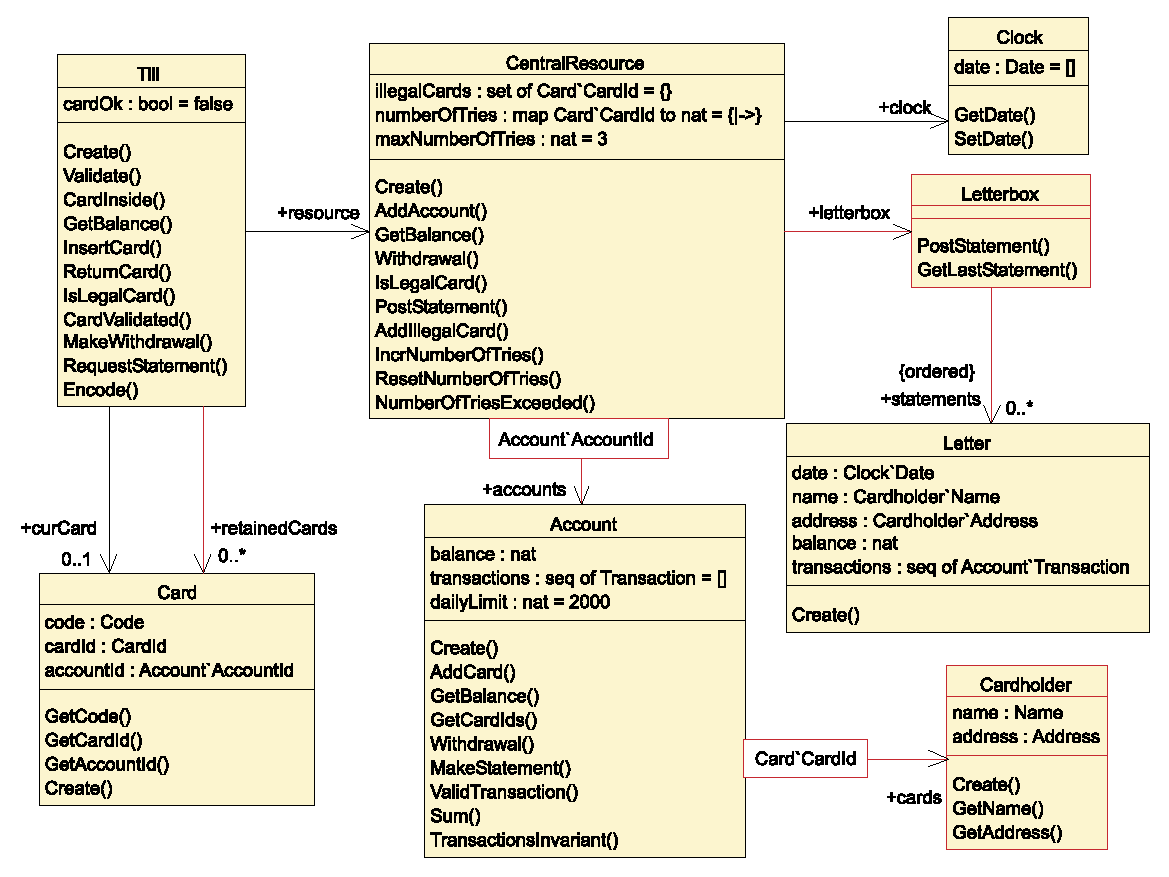
\includegraphics[width=.9\textwidth]{fullclassdiagram2}
\caption{Full overall UML class diagram.\label{fig:VDM++full}}
\end{center}
\end{figure}

The OO model is validated in the same fashion as the VDM-SL model, 
i.e. by the specifier and the client. The client interacts with 
the same front-end, except that it is now possible to add new 
tills (see Figure~\ref{fig:ppscreen}). In addition, we have developed a test environment for 
more systematic testing of the VDM++ specification. This is executed 
automatically using a number of batch scripts interacting with 
a command line version of \vdmtools. While running 
the test environment \vdmtools\  can collect test 
coverage and statistics information. Moreover, the pretty-printer 
can colour non-executed parts and insert a table of test statistics in 
the pretty-printed document. This is illustrated in
Appendix~\ref{app:VDMPP}.
The \texttt{\emph{Till}} class is fully covered by the test, but the
\texttt{\emph{CentralResource}}
class is not. Non-covered parts are printed using a user-specified
font, in this case grey. 


\begin{figure}[htbp]
\begin{center}
\includegraphics[width=.9\textwidth]{ppscreen}
\caption{Prototype GUI for VDM++ model.\label{fig:ppscreen}}
\end{center}
\end{figure}

\section{Concurrent VDM++ Model}\label{sec:Concur}


An enhancement to the VDM++ model is to consider each till as an
independent thread which executes concurrently with the other
tills. Further, we wish to be able to model the communication
behaviour between a till and the central resource, and in particular
model the possible failure of the communication channel between
them. All of these properties are captured in the final model, which
is also in VDM++ but is thread based. This model was tested in a
number of different scenarios using an extension of \vdmtools\ with
more support for development of real-time systems
\cite{GuidelinesRT,Mukherjee&00}.  The concurrent model is using
periodic threads which cannot be interpreted in the standard
interpreter from \vdmtools\ because there is no notion of time
included. The extension with real-time support has incorporated time
and it is avaiable in a beta-release form from IFAD's web pages
\cite{IFADweb}.

To allow several concurrent \texttt{\emph{Till}} threads to
simultaneously access the central resource, the communication between
each \texttt{\emph{Till}} and the central resource needs to be made
asynchronous. This is consistent with both reality and also with the
desire to model possible failure in communication.

The overview of the communications architecture is in the UML class
diagram in Figure~\ref{fig:communication}. Of course this is only a
part of the overall UML diagram. However this diagram can be thought
of as being a direct replacement for the assocation between
\texttt{\emph{Till}} and
\texttt{\emph{CentralResource}} 
in the previous class diagram.

\begin{figure}[htbp]
\begin{center}
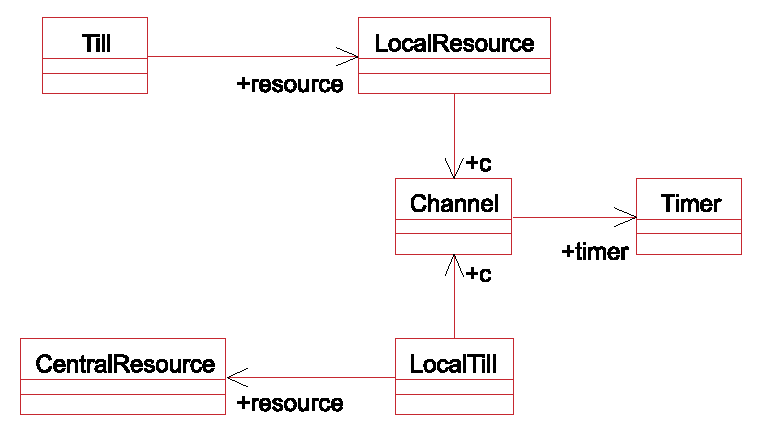
\includegraphics[width=4.487in]{communicationview2}
\caption{Communications view in UML.\label{fig:communication}}
\end{center}
\end{figure}

The classes \texttt{\emph{LocalResource}} and
\texttt{\emph{LocalTill}} are wrappers which allow the previous VDM++
model to be extended with minimum modifications to existing classes
(in fact only the \texttt{\emph{Till}} class is modified, as we
explain below). \texttt{\emph{Channel}} is a one place buffer which models the
communication between the \texttt{\emph{Till}} and the
\texttt{\emph{CentralResource}}.  The \texttt{\emph{Channel}} has a
timer which is used to measure whether the amount of time that the
channel has been waiting for a response from the
\texttt{\emph{CentralResource}} exceeds some predefined amount. This
is used to model failure of the communication channel.

To facilitate this architecture, a number of threads exist:
\texttt{\emph{Channel}} has its own thread which ensures that
\texttt{\emph{Till}} always receives a response to requests to the
\texttt{\emph{CentralResource}} within a fixed period.  The
\texttt{\emph{Timer}} class has its own thread,to update its clock,
and \texttt{\emph{LocalTill}} has its own thread, which checks whether
any messages have arrived on the \texttt{\emph{Channel}} from a
\texttt{\emph{Till}}. Consistency of shared objects (e.g.  the
\texttt{\emph{Channel}}) is ensured by the use of \textit{permission
predicates} which formally specify the circumstances in which an operation 
of a shared object may be invoked.

Although only one \texttt{\emph{Till}} is shown in the diagram, there
can in fact be any number of \texttt{\emph{Till}}s connected to the
\texttt{\emph{CentralResource}}.  For each such \texttt{\emph{Till}},
there would be a separate \texttt{\emph{LocalTill}},
\texttt{\emph{Channel}}, \texttt{\emph{Timer}} and
\texttt{\emph{LocalResource}} object. However all such tills
communicate with the same Central Resource.

The VDM++ model corresponding to this diagram is given in Appendix 
C. 


\section{Java Implementation}\label{sec:javaimpl}

Using \vdmtools\ the concurrent VDM++ model described in the previous
section was automatically translated into Java code, which could be
compiled without modification, and in conjunction with a driver class
could be executed. In addition to the driver thread, three threads
corresponding to the Channel, Timer and LocalTill threads are
created. In addition the permission predicates specified in the VDM++
model are also generated, ensuring that the synchronization properties
specified in the formal model are preserved in the Java
implementation. The code generated Java model was tested in a number
of different scenarios and demonstrated using the same GUI as was used
for the two different VDM++ models.


\section{Concluding Remarks}\label{sec:conclude}

This extended example of the use of \vdmtools\ has demonstrated a
number of key facets of this technology. We briefly summarise each of
these now.  

The initial VDM-SL model captured the high-level requirements. Using a
graphical front-end connected to the model using \vdmtools\ API, it was
possible to discuss this interpretation of the requirements with the
customer, allowing the resolution of any differences or
misunderstandings. Because of the use of the graphical front-end, this
discussion can take place independent of the formal notation used,
meaning that the customer can see the the requirements in a familiar
yet precise way, rather than as a formal specification or a use
case. Thus this approach leads to a significant reduction in the risk
of any misunderstanding between the customer and developer.

 From the VDM-SL model, a VDM++ model was developed, in conjunction
with a UML model using the round trip engineering features of
\vdmtools. The VDM++ model was then thoroughly tested using the
execution and test coverage features of \vdmtools. This kind of
searching analysis was only possible because of the precise and yet
abstract manner in which VDM++ models are described. In contrast a UML
model by itself would not allow such detailed analysis, while
analysing program code at this stage would make it difficult to focus
on critical aspects of the design. Hence this approach reduces the
risk of erroneous design.

 From the VDM++ model, a concurrent VDM++ model was developed,
facilitating modeling of communication between tills and the central
resource, including simulation of failure of communication.

Finally, from the VDM++ model, Java code was automatically
generated. Of course, the ability to click a button to generate
production quality code leads to a drastic reduction in the length of
the coding phase. Moreover use of automatic code generation means that
there is an exact correspondance between the model and code, making it
easier to understand the behaviour of the code. It also means that
test suites used to test the design can be reused on the code.

Throughout the example, the emphasis has been to apply formal methods
technology in a pragmatic manner, allowing straightforward integration
of such technology into an organisation's existing development
process. Nonetheless, as demonstrated this technology can lead to real
reduction in project risk, and an overall reduction in development
time. 

\bibliographystyle{iptes}

\bibliography{ifad}

\appendix

\newpage
\section{VDM-SL Model}\label{app:VDMSL}

In this model we assume there is one central resource and one 
till. Hence, there is no concurrency related to tills, but, for 
example, it is possible to report a card is illegal in the central 
resource while the card is in use at the till. This situation is 
handled using pre-conditions on operations. The purpose of the 
model is to analyze the main data and functional aspects of the 
system, e.g. ensuring that the daily limit is not exceeded and 
that cards are properly validated. 

The state of the model holds accounts and illegal cards associated 
with the central resource and current card and retained cards 
associated with the till. The \texttt{\emph{cardOk}} variable records whether 
or not a card has been validated successfully. 

\begin{VDMgray}
\textbf{state} \textit{System} \textbf{of}
 \textit{accounts} : \textbf{map} \textit{AccountId} \textbf{to} \textit{Account}
 \textit{illegalCards} : \textbf{set} \textbf{of} \textit{CardId}
 \textit{curCard} : \ensuremath{[}\textit{Card}\ensuremath{]}
 \textit{cardOk} : \textbf{bool}
 \textit{retainedCards} : \textbf{set} \textbf{of} \textit{Card}
\textbf{inv} \textbf{mk\_}\textit{System}(\textit{accs},-,\textit{curCard},\textit{cardOk},-) ==
   (\textit{curCard} = \textbf{nil} =\texttt{>} \textbf{not} \textit{cardOk}) \textbf{and}
   (\textbf{forall} \textit{id1}, \textit{id2} \textbf{in set} \textbf{dom} \textit{accs} \&
        \textit{id1} \texttt{<}\texttt{>} \textit{id2} =\texttt{>}
        \textbf{dom} \textit{accs}(\textit{id1}).\textit{cards} \textbf{inter}
        \textbf{dom} \textit{accs}(\textit{id2}).\textit{cards} = \{\})
\textbf{init} \textit{s} == \textit{s} = \textbf{mk\_}\textit{System}(\{{\textbar}-\texttt{>}\},\{\},\textbf{nil},\textbf{false},\{\})
\textbf{end}
\end{VDMgray}

The invariant on the state ensures that card ids are unique across 
accounts. The main data values of the model are defined as the 
following types.

\begin{VDMgray}
\textbf{types}
 \textit{Account} :: \textit{cards} : \textbf{map} \textit{CardId} \textbf{to} \textit{Cardholder}
            \textit{balance} : \textbf{nat}
            \textit{transactions} : \textbf{seq} \textbf{of} \textit{Transaction}
 \textbf{inv} \textit{account} == 
        \textit{TransactionsInvariant}(\textit{account}.\textit{transactions});
\end{VDMgray}


The invariant on account ensures that the daily limit is not 
exceeded. Due to the use of a mapping type for cards, it is ensured 
that card ids are unique for each account. We assume that it 
should not be possible to have a negative balance on an account, 
and the \texttt{\emph{Withdrawal}} operation below ensures that this does not 
happen. This is an issue of the credit policy from the bank towards
its customers so this must naturally be discussed.

\begin{VDMgray}
 \textit{Transaction} :: \textit{date} : \textit{Date}
                \textit{cardId} : \textit{CardId}
                \textit{amount} : \textbf{nat};
\end{VDMgray}


A transaction is modelled as a record structure, holding a date 
of the transaction, the card used to perform the transaction 
and the amount withdrawn.

\begin{VDMgray}
 \textit{Card} :: \textit{code} : \textit{Code}
         \textit{cardId} : \textit{CardId}
         \textit{accountId} : \textit{AccountId};
\end{VDMgray}


A card has a code, a card id and an account id. Below some of 
the simpler data types are defined.

\begin{VDMgray}
 \textit{Cardholder} :: \textit{name} : \textit{Name};

 \textit{AccountId} = \textbf{nat};
 \textit{Address} = \textbf{seq} \textbf{of} \textbf{char};
 \textit{Name} = \textbf{seq} \textbf{of} \textbf{char};
 \textit{CardId} = \textbf{nat};
 \textit{Code} = \textbf{nat};
 \textit{PinCode} = \textbf{nat};
 \textit{Date} = \textbf{seq} \textbf{of} \textbf{char};

\textbf{functions}
\end{VDMgray}


The following definitions introduces the auxiliary function for 
the invariant on account.

\begin{VDMgray}
 \textit{TransactionsInvariant} : \textbf{seq} \textbf{of} \textit{Transaction} +\texttt{>} \textbf{bool}
 \textit{TransactionsInvariant}(\textit{ts}) ==
 \textbf{forall} \textit{date} \textbf{in set} \{\textit{ts}(\textit{i}).\textit{date} {\textbar} \textit{i} \textbf{in set} \textbf{inds} \textit{ts}\} \&
        \textit{DateTotal}(\textit{date},\textit{ts}) \texttt{<}= \textit{dailyLimit};

 \textit{DateTotal} : \textit{Date} * \textbf{seq} \textbf{of} \textit{Transaction} +\texttt{>} \textbf{nat}
 \textit{DateTotal}(\textit{date},\textit{ts}) ==
   \textit{Sum}(\ensuremath{[}\textit{ts}(\textit{i}).\textit{amount} {\textbar} \textit{i} \textbf{in set} \textbf{inds} \textit{ts} 
                    \& \textit{ts}(\textit{i}).\textit{date} = \textit{date}\ensuremath{]});
\end{VDMgray}


The daily limit on withdrawals is a constant value, which in 
this model is set to an arbitrary value to be agreed with our customer
about. 

\begin{VDMgray}
\textbf{values}
 \textit{dailyLimit} : \textbf{nat} = 2000;

\textbf{operations}
\end{VDMgray}


The \texttt{\emph{InsertCard}} operation models the activity of
inserting a card into the till. This cannot be done if the till holds
a card already.  This is documented in the pre-condition.

\begin{VDMgray}
 \textit{InsertCard} : \textit{Card} ==\texttt{>} ()
 \textit{InsertCard}(\textit{c}) ==
   \textit{curCard} := \textit{c}
 \textbf{pre} \textit{curCard} = \textbf{nil};
\end{VDMgray}


The operation \texttt{\emph{Validate}} is used to validate a PIN code and to 
check that a card is not illegal. The pre-condition ensures that 
the till currently holds a card that has not already been validated. 
If a card turns out to be illegal, the machine retains the card. 

\begin{VDMgray}
 \textit{Validate} : \textit{PinCode} ==\texttt{>} \texttt{<}PinOk\texttt{>} {\textbar} \texttt{<}PinNotOk\texttt{>} {\textbar} \texttt{<}Retained\texttt{>}
 \textit{Validate}(\textit{pin}) ==
   \textbf{let} \textit{codeOk} = \textit{curCard}.\textit{code} = \textit{Encode}(\textit{pin}),
       \textit{cardLegal} = \textit{IsLegalCard}(\textit{curCard})
   \textbf{in}
     (\textbf{if} \textbf{not} \textit{cardLegal} \textbf{then}
       (\textit{retainedCards} := \textit{retainedCards} \textbf{union} \{\textit{curCard}\};
        \textit{cardOk} := \textbf{false};
        \textit{curCard} := \textbf{nil};
        \textbf{return} \texttt{<}Retained\texttt{>})
      \textbf{else}
        \textit{cardOk} := \textit{codeOk};
     \textbf{return} \textbf{if} \textit{cardOk}
            \textbf{then} \texttt{<}PinOk\texttt{>}
            \textbf{else} \texttt{<}PinNotOk\texttt{>})
 \textbf{pre} \textit{curCard} \texttt{<}\texttt{>} \textbf{nil} \textbf{and} \textbf{not} \textit{cardOk};
\end{VDMgray}


The \texttt{\emph{ReturnCard}} operation is useful to end user sessions, though 
it is not mentioned in the requirements. It allows the user to 
perform more than one transaction in each session, e.g. to first 
view the balance and then make a withdrawal.

\begin{VDMgray}
 \textit{ReturnCard} : () ==\texttt{>} ()
 \textit{ReturnCard}() ==
   (\textit{cardOk} := \textbf{false};
    \textit{curCard}:= \textbf{nil})
 \textbf{pre} \textit{curCard} \texttt{<}\texttt{>} \textbf{nil};
\end{VDMgray}


The following three operations correspond to the required functions
listed in the informal requirement description from
Section~\ref{sec:req}. They all require that the till holds a card
which has been validated successfully and not reported illegal.

\begin{VDMgray}
 \textit{GetBalance} : () ==\texttt{>} \textbf{nat}
 \textit{GetBalance}() ==
   \textbf{return} \textit{accounts}(\textit{curCard}.\textit{accountId}).\textit{balance}
 \textbf{pre} \textit{curCard} \texttt{<}\texttt{>} \textbf{nil} \textbf{and} \textit{cardOk} \textbf{and} \textit{IsLegalCard}(\textit{curCard});
\end{VDMgray}


The \texttt{\emph{MakeWithdrawal}} operation checks two things, that accounts are 
not overdrawn and that the daily limit is not exceeded. 

\begin{VDMgray}
 \textit{MakeWithdrawal} : \textbf{nat} * \textit{Date} ==\texttt{>} \textbf{bool}
 \textit{MakeWithdrawal}(\textit{amount},\textit{date}) ==
   \textbf{let} \textbf{mk\_}\textit{Card}(-,\textit{cardId},\textit{accountId}) = \textit{curCard},
       \textit{transaction} = \textbf{mk\_}\textit{Transaction}(\textit{date},\textit{cardId},\textit{amount})
   \textbf{in}
     \textbf{if} \textit{accounts}(\textit{accountId}).\textit{balance} - \textit{amount} \texttt{>}= 0 \textbf{and}
        \textit{DateTotal}(\textit{date},\textit{accounts}(\textit{accountId}).\textit{transactions}{\textasciicircum}
	               \ensuremath{[}\textit{transaction}\ensuremath{]})
          \texttt{<}= \textit{dailyLimit}
     \textbf{then}
        (\textit{accounts}(\textit{accountId}).\textit{balance} :=
            \textit{accounts}(\textit{accountId}).\textit{balance} - \textit{amount};
         \textit{accounts}(\textit{accountId}).\textit{transactions} :=
            \textit{accounts}(\textit{accountId}).\textit{transactions} 
             {\textasciicircum} \ensuremath{[}\textit{transaction}\ensuremath{]};
         \textbf{return} \textbf{true})
     \textbf{else}
         \textbf{return} \textbf{false}
 \textbf{pre} \textit{curCard} \texttt{<}\texttt{>} \textbf{nil} \textbf{and} \textit{cardOk} \textbf{and} \textit{IsLegalCard}(\textit{curCard});
\end{VDMgray}


The following operation returns a simple account statement, which 
can be sent to a cardholder.

\begin{VDMgray}
 \textit{RequestStatement} : () ==\texttt{>} \textit{Name} * \textbf{seq} \textbf{of} \textit{Transaction} * \textbf{nat}
 \textit{RequestStatement}() ==
   \textbf{let} \textbf{mk\_}\textit{Card}(-,\textit{cardId},\textit{accountId}) = \textit{curCard},
       \textbf{mk\_}\textit{Account}(\textit{cards},\textit{balance},\textit{transactions}) =
                  \textit{accounts}(\textit{accountId})
   \textbf{in}
     \textbf{return} \textbf{mk\_}(\textit{cards}(\textit{cardId}).\textit{name},\textit{transactions},\textit{balance})
 \textbf{pre} \textit{curCard} \texttt{<}\texttt{>} \textbf{nil} \textbf{and} \textit{cardOk} \textbf{and} \textit{IsLegalCard}(\textit{curCard});
\end{VDMgray}


A card is legal if it has not been reported illegal, its account 
id is valid, and its card id is valid.

\begin{VDMgray}
 \textit{IsLegalCard} : \textit{Card} ==\texttt{>} \textbf{bool}
 \textit{IsLegalCard}(\textbf{mk\_}\textit{Card}(-,\textit{cardId},\textit{accountId})) ==
   \textbf{return} \textit{cardId} \textbf{not in set} \textit{illegalCards} \textbf{and}
          \textit{accountId} \textbf{in set} \textbf{dom} \textit{accounts} \textbf{and}
          \textit{cardId} \textbf{in set} \textbf{dom} \textit{accounts}(\textit{accountId}).\textit{cards};
\end{VDMgray}


The following operations are provided to update the accounts 
and illegal cards. 

\begin{VDMgray}
 \textit{ReportIllegalCard} : \textit{CardId} ==\texttt{>} ()
 \textit{ReportIllegalCard}(\textit{cardId}) ==
   \textit{illegalCards} := \textit{illegalCards} \textbf{union} \{\textit{cardId}\};

 \textit{AddAccount} : \textit{AccountId} * \textit{Account} ==\texttt{>} ()
 \textit{AddAccount}(\textit{accountId},\textit{account}) ==
   \textit{accounts} := \textit{accounts} \textbf{munion} \{\textit{accountId} {\textbar}-\texttt{>} \textit{account}\}
 \textbf{pre} \textit{accountId} \textbf{not in set} \textbf{dom} \textit{accounts};
\end{VDMgray}


Finally we define two auxiliary functions. Note that we have 
not decided on a concrete encoding function.

\begin{VDMgray}
\textbf{functions}
 \textit{Encode}: \textit{PinCode} +\texttt{>} \textit{Code}
 \textit{Encode}(\textit{pin}) ==
   \textit{pin};
   -- The actual encoding procedure has not yet been chosen

 \textit{Sum}: \textbf{seq} \textbf{of} \textbf{real} +\texttt{>} \textbf{real}
 \textit{Sum}(\textit{rs}) ==
 \textbf{if} \textit{rs} = \ensuremath{[}\ensuremath{]} \textbf{then} 0
 \textbf{else} \textbf{hd} \textit{rs} + \textit{Sum}(\textbf{tl} \textit{rs});
\end{VDMgray}

\newpage
\section{The UML/VDM++ Model}\label{app:VDMPP}

Having demonstrated the VDM-SL model to the ``imaginary'' customer we
now produce a more design-oriented UML/VDM++ model of the
``cash-point'' service system. This model copes with multiple tills
and includes structuring of the model in terms of classes and
associations between them. Figure~\ref{fig:VDM++full} on
page~\pageref{fig:VDM++full} shows the main
class diagram for the UML/VDM++ model.

The overall system then has a number of instances of the Till 
class and one CentralResource. It also has a clock 
and a collections of cards which the customers use. The rest 
of this appendix lists the VDM++ classes, which are documented 
in RTF files read into \vdmtools. The test coverage 
facility is used to illustrate the extent to which we have systematically 
tested the VDM++ model. It is deliberately not fully tested in 
order to illustrate how this is documented using
\vdmtools. 

\subsection{The Class Till}

This class models a till. A till is connected to a central resource 
and holds a number of retained cards, which have not been returned 
to a user of the till. It may hold a current card and it has 
an attribute to say whether the current card and its PIN code 
have been validated successfully. In this version of the till 
we assume that the central resource will always become available 
within a reasonable time limit.

\begin{VDMgray}
\textbf{class} \textit{Till}

\textbf{instance} \textbf{variables}
 \textit{curCard} : \ensuremath{[}\textit{Card}\ensuremath{]} := \textbf{nil};
 \textit{cardOk} : \textbf{bool} := \textbf{false};
 \textit{retainedCards} : \textbf{set} \textbf{of} \textit{Card} := \{\};
 \textit{resource} : \textit{CentralResource};
 \textbf{inv} \textit{curCard} = \textbf{nil} =\texttt{>} \textbf{not} \textit{cardOk};
\end{VDMgray}


The invariant says that if there is no card in the till then 
the validation status of the current card shall be false.

\begin{VDMgray}
\textbf{operations}
 \textbf{public}
 \textit{Create}: \textit{CentralResource} ==\texttt{>} \textit{Till}
 \textit{Create}(\textit{res}) ==
   (\textit{resource} := \textit{res};
    \textbf{return} \textbf{self});
\end{VDMgray}

The \texttt{\emph{Create}} operation is used once in a till object's lifetime 
in order to set up a connection to a central resource.

\begin{VDMgray}
 \textbf{public}
 \textit{InsertCard} : \textit{Card} ==\texttt{>} ()
 \textit{InsertCard}(\textit{c}) ==
   \textit{curCard} := \textit{c}
 \textbf{pre} \textbf{not} \textit{CardInside}();
\end{VDMgray}


The \texttt{\emph{InsertCard}} operation models the activity of inserting a card 
into the till. This cannot be done if the till holds a card already, 
which is documented in the pre-condition.

\begin{VDMgray}
 \textbf{public}
 \textit{Validate} : \textit{Card}\`{}\textit{PinCode} ==\texttt{>} \texttt{<}PinOk\texttt{>} {\textbar} \texttt{<}PinNotOk\texttt{>} 
                             {\textbar} \texttt{<}Retained\texttt{>}
 \textit{Validate}(\textit{pin}) ==
   \textbf{let} \textit{cardId} = \textit{curCard}.\textit{GetCardId}(),
       \textit{codeOk} = \textit{curCard}.\textit{GetCode}() = \textit{Encode}(\textit{pin}),
       \textit{cardLegal} = \textit{IsLegalCard}()
   \textbf{in}
     (\textit{cardOk} := \textit{codeOk} \textbf{and} \textit{cardLegal};
      \textbf{if} \textbf{not} \textit{cardLegal} \textbf{then}
          (\textit{retainedCards} := \textit{retainedCards} \textbf{union} \{\textit{curCard}\};
           \textit{curCard} := \textbf{nil};
           \textbf{return} \texttt{<}Retained\texttt{>})
      \textbf{elseif} \textit{codeOk} \textbf{then}
           \textit{resource}.\textit{ResetNumberOfTries}(\textit{cardId})
      \textbf{else} (\textit{resource}.\textit{IncrNumberOfTries}(\textit{cardId});
            \textbf{if} \textit{resource}.\textit{NumberOfTriesExceeded}(\textit{cardId}) \textbf{then}
              (\textit{retainedCards} := \textit{retainedCards} \textbf{union}
	                                 \{\textit{curCard}\};
               \textit{cardOk} := \textbf{false};
               \textit{curCard} := \textbf{nil};
               \textbf{return} \texttt{<}Retained\texttt{>}));
      \textbf{return} \textbf{if} \textit{cardOk}
             \textbf{then} \texttt{<}PinOk\texttt{>}
             \textbf{else} \texttt{<}PinNotOk\texttt{>})
 \textbf{pre} \textit{CardInside}() \textbf{and} \textbf{not} \textit{cardOk};
\end{VDMgray}


The \texttt{\emph{Validate}} operation is used to validate a PIN code and to 
check that a card is not illegal. The pre-condition ensures that 
the till currently holds a card which has not yet been validated. 
If a card turns out to be illegal, the machine keeps the card. 


\begin{VDMgray}
 \textbf{public}
 \textit{ReturnCard} : () ==\texttt{>} ()
 \textit{ReturnCard}() ==
   (\textit{cardOk} := \textbf{false};
    \textit{curCard}:= \textbf{nil})
 \textbf{pre} \textit{CardInside}();
\end{VDMgray}


The \texttt{\emph{ReturnCard}} operation is useful to end user sessions, though 
it is not mentioned in the requirements. It allows the user to 
perform more than one transaction in each session, e.g. to first 
view the balance and then make a withdrawal.

The following three operations are listed in the requirements 
document. They all require that the till holds a card which has 
been validated successfully. The operations are mirrored in the 
central resource. The \texttt{\emph{GetBalance}} operation return the value \texttt{\emph{nil}} 
if it is not possible to get the balance. 

\begin{VDMgray}
 \textbf{public}
 \textit{GetBalance} : () ==\texttt{>} \ensuremath{[}\textbf{nat}\ensuremath{]}
 \textit{GetBalance}() ==
   \textit{resource}.\textit{GetBalance}(\textit{curCard}.\textit{GetAccountId}())
 \textbf{pre} \textit{CardValidated}();
\end{VDMgray}


The \texttt{\emph{MakeWithdrawal}} and \texttt{\emph{RequestStatement}} operations each return 
a boolean indicating whether the requested transactions could 
be completed.

\begin{VDMgray}
 \textbf{public}
 \textit{MakeWithdrawal} : \textbf{nat} ==\texttt{>} \textbf{bool}
 \textit{MakeWithdrawal}(\textit{amount}) ==
   \textit{resource}.\textit{Withdrawal}(\textit{curCard}.\textit{GetAccountId}(),
                       \textit{curCard}.\textit{GetCardId}(),\textit{amount})
 \textbf{pre} \textit{CardValidated}();

 \textbf{public}
 \textit{RequestStatement} : () ==\texttt{>} \textbf{bool}
 \textit{RequestStatement}() ==
   \textit{resource}.\textit{PostStatement}(\textit{curCard}.\textit{GetAccountId}(),
                          \textit{curCard}.\textit{GetCardId}())
 \textbf{pre} \textit{CardValidated}();
\end{VDMgray}


The \texttt{\emph{IsLegalCard}} operation below is only used internally to validate 
a card.

\begin{VDMgray}
 \textbf{public}
 \textit{IsLegalCard} : () ==\texttt{>} \textbf{bool}
 \textit{IsLegalCard}() ==
   \textbf{return} \textit{resource}.\textit{IsLegalCard}(\textit{curCard}.\textit{GetAccountId}(),
                               \textit{curCard}.\textit{GetCardId}())
 \textbf{pre} \textit{CardInside}();

 \textbf{public}
 \textit{CardValidated}: () ==\texttt{>} \textbf{bool}
 \textit{CardValidated}() ==
   \textbf{return} \textit{curCard} \texttt{<}\texttt{>} \textbf{nil} \textbf{and} \textit{cardOk};

 \textbf{public}
 \textit{CardInside}: () ==\texttt{>} \textbf{bool}
 \textit{CardInside}() ==
   \textbf{return} \textit{curCard} \texttt{<}\texttt{>} \textbf{nil};

\textbf{functions}
\end{VDMgray}


The requirements say that the till should encode the PIN code 
before comparing it to the code on the card. We have documented 
this requirement in the function below, but not yet made a choice 
of approach to this.

\begin{VDMgray}
 \textit{Encode}: \textit{Card}\`{}\textit{PinCode} +\texttt{>} \textit{Card}\`{}\textit{Code}
 \textit{Encode}(\textit{pin}) ==
   \textit{pin};
   -- The actual encoding procedure has not yet been chosen

\textbf{end} \textit{Till}
\end{VDMgray}


The table below presents test coverage information for the Till 
class.

\begin{longtable}{lll}
\hline
\endhead
\hline
\endfoot
\multicolumn{1}{|p{3.086in}|}
{\raggedright
\textbf{\textit{name}}} & 
\multicolumn{1}{p{0.660in}|}
{\raggedright
\textbf{\textit{\#calls}}} & 
\multicolumn{1}{p{0.754in}|}
{\raggedright
\textbf{\textit{coverage}}}\\
\cline{1-1}\cline{2-2}\cline{3-3}
\multicolumn{1}{|p{3.086in}|}
{\raggedright
Till\`{}CardInside } & 
\multicolumn{1}{p{0.660in}|}
{\raggedright
  29 } & 
\multicolumn{1}{p{0.754in}|}
{\raggedright
100\%}\\
\cline{1-1}\cline{2-2}\cline{3-3}
\multicolumn{1}{|p{3.086in}|}
{\raggedright
Till\`{}CardValidated } & 
\multicolumn{1}{p{0.660in}|}
{\raggedright
  11 } & 
\multicolumn{1}{p{0.754in}|}
{\raggedright
100\%}\\
\cline{1-1}\cline{2-2}\cline{3-3}
\multicolumn{1}{|p{3.086in}|}
{\raggedright
Till\`{}Create } & 
\multicolumn{1}{p{0.660in}|}
{\raggedright
  24 } & 
\multicolumn{1}{p{0.754in}|}
{\raggedright
100\%}\\
\cline{1-1}\cline{2-2}\cline{3-3}
\multicolumn{1}{|p{3.086in}|}
{\raggedright
Till\`{}Encode } & 
\multicolumn{1}{p{0.660in}|}
{\raggedright
  9 } & 
\multicolumn{1}{p{0.754in}|}
{\raggedright
100\%}\\
\cline{1-1}\cline{2-2}\cline{3-3}
\multicolumn{1}{|p{3.086in}|}
{\raggedright
Till\`{}GetBalance } & 
\multicolumn{1}{p{0.660in}|}
{\raggedright
  1 } & 
\multicolumn{1}{p{0.754in}|}
{\raggedright
100\%}\\
\cline{1-1}\cline{2-2}\cline{3-3}
\multicolumn{1}{|p{3.086in}|}
{\raggedright
Till\`{}InsertCard } & 
\multicolumn{1}{p{0.660in}|}
{\raggedright
  8 } & 
\multicolumn{1}{p{0.754in}|}
{\raggedright
100\%}\\
\cline{1-1}\cline{2-2}\cline{3-3}
\multicolumn{1}{|p{3.086in}|}
{\raggedright
Till\`{}IsLegalCard } & 
\multicolumn{1}{p{0.660in}|}
{\raggedright
  9 } & 
\multicolumn{1}{p{0.754in}|}
{\raggedright
100\%}\\
\cline{1-1}\cline{2-2}\cline{3-3}
\multicolumn{1}{|p{3.086in}|}
{\raggedright
Till\`{}MakeWithdrawal } & 
\multicolumn{1}{p{0.660in}|}
{\raggedright
  1 } & 
\multicolumn{1}{p{0.754in}|}
{\raggedright
100\%}\\
\cline{1-1}\cline{2-2}\cline{3-3}
\multicolumn{1}{|p{3.086in}|}
{\raggedright
Till\`{}RequestStatement } & 
\multicolumn{1}{p{0.660in}|}
{\raggedright
  2 } & 
\multicolumn{1}{p{0.754in}|}
{\raggedright
100\%}\\
\cline{1-1}\cline{2-2}\cline{3-3}
\multicolumn{1}{|p{3.086in}|}
{\raggedright
Till\`{}ReturnCard } & 
\multicolumn{1}{p{0.660in}|}
{\raggedright
  1 } & 
\multicolumn{1}{p{0.754in}|}
{\raggedright
100\%}\\
\cline{1-1}\cline{2-2}\cline{3-3}
\multicolumn{1}{|p{3.086in}|}
{\raggedright
Till\`{}Validate } & 
\multicolumn{1}{p{0.660in}|}
{\raggedright
  9 } & 
\multicolumn{1}{p{0.754in}|}
{\raggedright
100\%}\\
\cline{1-1}\cline{2-2}\cline{3-3}
\multicolumn{1}{|p{3.086in}|}
{\raggedright
\textbf{\textit{total}}} & 
\multicolumn{1}{p{0.660in}|}
{\raggedright
} & 
\multicolumn{1}{p{0.754in}|}
{\raggedright
\textbf{\textit{100\% }}}\\
\hline
\end{longtable}

 

\subsection{The Class CentralResource}

This class models the central resource. We assume there is only 
one central resource in the system, though many tills can be 
connected to this. The central resource holds the accounts, ids 
of illegal cards, and connections to a clock and a letterbox.

\begin{VDMgray}
\textbf{class} \textit{CentralResource}

\textbf{instance} \textbf{variables}
 \textit{accounts} : \textbf{map} \textit{Account}\`{}\textit{AccountId} \textbf{to} \textit{Account} := \{{\textbar}-\texttt{>}\};
 \textit{numberOfTries} : \textbf{map} \textit{Card}\`{}\textit{CardId} \textbf{to} \textbf{nat} := \{{\textbar}-\texttt{>}\};
 \textit{illegalCards} : \textbf{set} \textbf{of} \textit{Card}\`{}\textit{CardId} := \{\};
 \textit{letterbox} : \textit{Letterbox};
 \textit{clock} : \textit{Clock};
\end{VDMgray}


All cards for different accounts cannot be overlapping.

\begin{VDMgray}
 \textbf{inv} \textbf{forall} \textit{acc1},\textit{acc2} \textbf{in set} \textbf{rng} \textit{accounts} \&
            \textit{acc1} \texttt{<}\texttt{>} \textit{acc2} =\texttt{>}
            \textit{acc1}.\textit{GetCardIds}() \textbf{inter} \textit{acc2}.\textit{GetCardIds}() = \{\};
\end{VDMgray}

A constant has been defined for the maximum number of tries for a card
holder. This number must naturally also be discussed with the bank.

\begin{VDMgray}
\textbf{values}
 \textit{maxNumberOfTries} : \textbf{nat} = 3;
\end{VDMgray}

The \texttt{\emph{Create}} operation is used once in the lifetime for
the \texttt{\emph{CentralResource}}.

\begin{VDMgray}
\textbf{operations}
 \textbf{public}
 \textit{Create} : \textit{Clock} * \textit{Letterbox} ==\texttt{>} \textit{CentralResource}
 \textit{Create}(\textit{c},\textit{l}) ==
   (\textit{clock} := \textit{c};
    \textit{letterbox} := \textit{l};
    \textbf{return} \textbf{self});
\end{VDMgray}


The following three operations provide the functionality requested 
in the requirements specification of the system. The operations 
first check that the requested functionality is allowed and then 
hand the actual processing over to each account. Note that the 
checks are necessary even though the till may have performed 
them as well. For example, a card may have been reported stolen 
or illegal in another way while it is being used at a till. 

\begin{VDMgray}
 \textbf{public}
 \textit{GetBalance} : \textit{Account}\`{}\textit{AccountId} ==\texttt{>} \ensuremath{[}\textbf{nat}\ensuremath{]}
 \textit{GetBalance}(\textit{accountId}) ==
   \textbf{if} \textit{accountId} \textbf{in set} \textbf{dom} \textit{accounts} \textbf{then}
      \textit{accounts}(\textit{accountId}).\textit{GetBalance}()
   \textbf{else}{\color{color16} \textbf{return nil}};

 \textbf{public}
 \textit{Withdrawal} : \textit{Account}\`{}\textit{AccountId} * \textit{Card}\`{}\textit{CardId} * \textbf{nat} ==\texttt{>} \textbf{bool}
 \textit{Withdrawal}(\textit{accountId},\textit{cardId},\textit{amount}) ==
   \textbf{if} \textit{IsLegalCard}(\textit{accountId},\textit{cardId}) \textbf{then}
      \textit{accounts}(\textit{accountId}).
         \textit{Withdrawal}(\textit{cardId},\textit{amount},\textit{clock}.\textit{GetDate}())
   \textbf{else}{\color{color16} \textbf{return}} {\color{color16} \textbf{false}};

 \textbf{public}
 \textit{PostStatement} : \textit{Account}\`{}\textit{AccountId} * \textit{Card}\`{}\textit{CardId} ==\texttt{>} \textbf{bool}
 \textit{PostStatement}(\textit{accountId},\textit{cardId}) ==
   \textbf{if} \textit{IsLegalCard}(\textit{accountId},\textit{cardId}) \textbf{then}
      (\textit{letterbox}.\textit{PostStatement}(\textit{accounts}(\textit{accountId}).
         \textit{MakeStatement}(\textit{cardId},\textit{clock}.\textit{GetDate}()));
       \textbf{return} \textbf{true})
   \textbf{else}{\color{color16} \textbf{return}} {\color{color16} \textbf{false}};
\end{VDMgray}

Note how the else branches of the three operations have not yet been
covered with the chosen test cases. This is shown by colouring the
corresponding parts of teh VDM++ description in gray automatically by
the pretty printer for \vdmtools. 

Next some operations follow to check whether cards are legal 
and administer the number of tries stored for each card. 

\begin{VDMgray}
 \textbf{public}
 \textit{IsLegalCard} : \textit{Account}\`{}\textit{AccountId} * \textit{Card}\`{}\textit{CardId} ==\texttt{>} \textbf{bool}
 \textit{IsLegalCard}(\textit{accountId},\textit{cardId}) ==
   \textbf{return} \textit{cardId} \textbf{not in set} \textit{illegalCards} \textbf{and}
          \textit{accountId} \textbf{in set} \textbf{dom} \textit{accounts} \textbf{and}
          \textit{cardId} \textbf{in set} \textit{accounts}(\textit{accountId}).\textit{GetCardIds}();

 \textbf{public}
 \textit{NumberOfTriesExceeded} : \textit{Card}\`{}\textit{CardId} ==\texttt{>} \textbf{bool}
 \textit{NumberOfTriesExceeded}(\textit{cardId}) ==
   \textbf{return} \textit{numberOfTries}(\textit{cardId}) \texttt{>}= \textit{maxNumberOfTries};

 \textbf{public}
 \textit{ResetNumberOfTries} : \textit{Card}\`{}\textit{CardId} ==\texttt{>} ()
 \textit{ResetNumberOfTries}(\textit{cardId}) ==
   \textit{numberOfTries}(\textit{cardId}) := 0;

 \textbf{public}
 \textit{IncrNumberOfTries} : \textit{Card}\`{}\textit{CardId} ==\texttt{>} ()
 \textit{IncrNumberOfTries}(\textit{cardId}) ==
   \textit{numberOfTries}(\textit{cardId}) := \textit{numberOfTries}(\textit{cardId}) + 1;
\end{VDMgray}


The two operations below are used to update the central resource. 


\begin{VDMgray}
 \textbf{public}
 \textit{AddAccount} : \textit{Account}\`{}\textit{AccountId} * \textit{Account} ==\texttt{>} ()
 \textit{AddAccount}(\textit{accId},\textit{acc}) ==
   (\textit{numberOfTries} := \textit{numberOfTries} ++
                     \{\textit{cId} {\textbar}-\texttt{>} 0 {\textbar} \textit{cId} \textbf{in set} \textit{acc}.\textit{GetCardIds}()\};
    \textit{accounts} := \textit{accounts} ++ \{\textit{accId} {\textbar}-\texttt{>} \textit{acc}\})
 \textbf{pre} \textit{accId} \textbf{not in set} \textbf{dom} \textit{accounts};

 \textbf{public}
 \textit{AddIllegalCard} : \textit{Card}\`{}\textit{CardId} ==\texttt{>} ()
 \textit{AddIllegalCard}(\textit{cId}) ==
   \textit{illegalCards} := \textit{illegalCards} \textbf{union} \{\textit{cId}\};

\textbf{end} \textit{CentralResource}
\end{VDMgray}


The table below presents test coverage information for the
\texttt{\emph{CentralResource}}  class.

\begin{longtable}{lll}
\hline
\multicolumn{1}{|p{3.086in}|}
{\raggedright
\textbf{\textit{name}}} & 
\multicolumn{1}{p{0.660in}|}
{\raggedright
\textbf{\textit{\#calls}}} & 
\multicolumn{1}{p{0.754in}|}
{\raggedright
\textbf{\textit{coverage}}}\\
\cline{1-1}\cline{2-2}\cline{3-3}
\multicolumn{1}{|p{3.086in}|}
{\raggedright
CentralResource\`{}AddAccount } & 
\multicolumn{1}{p{0.660in}|}
{\raggedright
  40 } & 
\multicolumn{1}{p{0.754in}|}
{\raggedright
100\%}\\
\cline{1-1}\cline{2-2}\cline{3-3}
\multicolumn{1}{|p{3.086in}|}
{\raggedright
CentralResource\`{}AddIllegalCard } & 
\multicolumn{1}{p{0.660in}|}
{\raggedright
  1 } & 
\multicolumn{1}{p{0.754in}|}
{\raggedright
100\%}\\
\cline{1-1}\cline{2-2}\cline{3-3}
\multicolumn{1}{|p{3.086in}|}
{\raggedright
CentralResource\`{}Create } & 
\multicolumn{1}{p{0.660in}|}
{\raggedright
  8 } & 
\multicolumn{1}{p{0.754in}|}
{\raggedright
100\%}\\
\cline{1-1}\cline{2-2}\cline{3-3}
\multicolumn{1}{|p{3.086in}|}
{\raggedright
CentralResource\`{}GetBalance } & 
\multicolumn{1}{p{0.660in}|}
{\raggedright
  1 } & 
\multicolumn{1}{p{0.754in}|}
{\raggedright
81\%}\\
\cline{1-1}\cline{2-2}\cline{3-3}
\multicolumn{1}{|p{3.086in}|}
{\raggedright
CentralResource\`{}IncrNumberOfTries } & 
\multicolumn{1}{p{0.660in}|}
{\raggedright
  4 } & 
\multicolumn{1}{p{0.754in}|}
{\raggedright
100\%}\\
\cline{1-1}\cline{2-2}\cline{3-3}
\multicolumn{1}{|p{3.086in}|}
{\raggedright
CentralResource\`{}IsLegalCard } & 
\multicolumn{1}{p{0.660in}|}
{\raggedright
  12 } & 
\multicolumn{1}{p{0.754in}|}
{\raggedright
100\%}\\
\cline{1-1}\cline{2-2}\cline{3-3}
\multicolumn{1}{|p{3.086in}|}
{\raggedright
CentralResource\`{}NumberOfTriesExceeded } & 
\multicolumn{1}{p{0.660in}|}
{\raggedright
  4 } & 
\multicolumn{1}{p{0.754in}|}
{\raggedright
100\%}\\
\cline{1-1}\cline{2-2}\cline{3-3}
\multicolumn{1}{|p{3.086in}|}
{\raggedright
CentralResource\`{}PostStatement } & 
\multicolumn{1}{p{0.660in}|}
{\raggedright
  2 } & 
\multicolumn{1}{p{0.754in}|}
{\raggedright
90\%}\\
\cline{1-1}\cline{2-2}\cline{3-3}
\multicolumn{1}{|p{3.086in}|}
{\raggedright
CentralResource\`{}ResetNumberOfTries } & 
\multicolumn{1}{p{0.660in}|}
{\raggedright
  4 } & 
\multicolumn{1}{p{0.754in}|}
{\raggedright
100\%}\\
\cline{1-1}\cline{2-2}\cline{3-3}
\multicolumn{1}{|p{3.086in}|}
{\raggedright
CentralResource\`{}Withdrawal } & 
\multicolumn{1}{p{0.660in}|}
{\raggedright
  1 } & 
\multicolumn{1}{p{0.754in}|}
{\raggedright
87\%}\\
\cline{1-1}\cline{2-2}\cline{3-3}
\multicolumn{1}{|p{3.086in}|}
{\raggedright
\textbf{\textit{total}}} & 
\multicolumn{1}{p{0.660in}|}
{\raggedright
} & 
\multicolumn{1}{p{0.754in}|}
{\raggedright
\textbf{\textit{94\% }}}\\
\hline
\end{longtable}

 
\subsection{The Class Account}

This class models an account. A number of cards held by individual 
cardholders are associated with an account. An account has a 
balance and records transactions.

\begin{VDMgray}
\textbf{class} \textit{Account}

\textbf{instance} \textbf{variables}
 \textit{cards} : \textbf{map} \textit{Card}\`{}\textit{CardId} \textbf{to} \textit{Cardholder};
 \textit{balance} : \textbf{nat};
 \textit{transactions} : \textbf{seq} \textbf{of} \textit{Transaction} := \ensuremath{[}\ensuremath{]};
 \textbf{inv} \textit{TransactionsInvariant}(\textit{transactions});
\end{VDMgray}


The invariant ensures that transactions performed on the same 
day do not exceed the daily limit, which is a constant value 
defined below. Note that we have chosen to not allow a negative 
balance. As mentioned above such an issue must naturally be discussed
with the bank. 

\begin{VDMgray}
\textbf{values}
 \textit{dailyLimit} : \textbf{nat} = 2000;

\textbf{types}
 \textbf{public} \textit{AccountId} = \textbf{nat};
 \textbf{public}
 \textit{Transaction} :: \textit{date} : \textit{Clock}\`{}\textit{Date}
                \textit{cardId} : \textit{Card}\`{}\textit{CardId}
                \textit{amount} : \textbf{nat};
\end{VDMgray}


In this specification we have chosen to model transaction as 
a type. Alternatively it could have been modelled as a class, 
but it has no obvious functionality except trivial read/write 
operations. Moreover, transaction objects/values do not need 
to be shared among many objects. Our choice also illustrates 
the power of the VDM++ type system.

\begin{VDMgray}
\textbf{operations}
 \textbf{public}
 \textit{Create} : \textbf{map} \textit{Card}\`{}\textit{CardId} \textbf{to} \textit{Cardholder} * \textbf{nat} ==\texttt{>} \textit{Account}
 \textit{Create}(\textit{cs},\textit{b}) ==
   (\textit{cards} := \textit{cs};
    \textit{balance} := \textit{b};
    \textbf{return} \textbf{self});

 \textbf{public}
 \textit{GetBalance} : () ==\texttt{>} \textbf{nat}
 \textit{GetBalance}() ==
   \textbf{return} \textit{balance};
\end{VDMgray}


The \texttt{\emph{Withdrawal}} operation checks that an account and the daily 
limit are not overdrawn. 

\begin{VDMgray}
 \textbf{public}
 \textit{Withdrawal} : \textit{Card}\`{}\textit{CardId} * \textbf{nat} * \textit{Clock}\`{}\textit{Date} ==\texttt{>} \textbf{bool}
 \textit{Withdrawal}(\textit{cardId},\textit{amount},\textit{date}) ==
   \textbf{let} \textit{transaction} = \textbf{mk\_}\textit{Transaction}(\textit{date},\textit{cardId},\textit{amount})
   \textbf{in}
     \textbf{if} \textit{balance} - \textit{amount} \texttt{>}= 0 \textbf{and}
        \textit{DateTotal}(\textit{date},\textit{transactions}{\textasciicircum}\ensuremath{[}\textit{transaction}\ensuremath{]}) 
        \texttt{<}= \textit{dailyLimit}
     \textbf{then}
        (\textit{balance} := \textit{balance} - \textit{amount};
         \textit{transactions} := \textit{transactions} {\textasciicircum} \ensuremath{[}\textit{transaction}\ensuremath{]};
         \textbf{return} \textbf{true})
     \textbf{else}{\color{color16} \textbf{return}} {\color{color16} \textbf{false}}
 \textbf{pre} \textit{cardId} \textbf{in set} \textbf{dom} \textit{cards};

 \textbf{public}
 \textit{MakeStatement} : \textit{Card}\`{}\textit{CardId} * \textit{Clock}\`{}\textit{Date} ==\texttt{>} \textit{Letter}
 \textit{MakeStatement}(\textit{cardId},\textit{date}) ==
   \textbf{let} \textit{nm} = \textit{cards}(\textit{cardId}).\textit{GetName}(),
       \textit{addr} = \textit{cards}(\textit{cardId}).\textit{GetAddress}()
   \textbf{in}
     (\textbf{dcl} \textit{letter} : \textit{Letter} := \textbf{new} Letter();
      \textit{letter}.\textit{Create}(\textit{nm},\textit{addr},\textit{date},\textit{transactions},\textit{balance}))
 \textbf{pre} \textit{cardId} \textbf{in set} \textbf{dom} \textit{cards};
\end{VDMgray}


The \texttt{\emph{GetCardIds}} operation is used to obtain all cards associated 
with the account.

\begin{VDMgray}
 \textbf{public}
 \textit{GetCardIds}: () ==\texttt{>} \textbf{set} \textbf{of} \textit{Card}\`{}\textit{CardId}
 \textit{GetCardIds}() ==
   \textbf{return} \textbf{dom} \textit{cards};
\end{VDMgray}


The following operations and functions provide auxiliary functionality 
of various sorts.

\begin{VDMgray}
 \textbf{public}
 \textit{AddCard} : \textit{Card}\`{}\textit{CardId} * \textit{Cardholder} ==\texttt{>} ()
 \textit{AddCard}(\textit{cId},\textit{ch}) ==
   {\color{color16} \textit{cards}} {\color{color16} :=} {\color{color16} \textit{cards}} {\color{color16} \textbf{munion}}{\color{color16} \{}{\color{color16} \textit{cId}} {\color{color16} {\textbar}-\texttt{>}} {\color{color16} \textit{ch}}{\color{color16} \}}
 \textbf{pre} {\color{color16} \textit{cId}} {\color{color16} \textbf{not in set}} {\color{color16} \textbf{dom}} {\color{color16} \textit{cards}};

\textbf{functions}
 \textit{TransactionsInvariant}: \textbf{seq} \textbf{of} \textit{Transaction} +\texttt{>} \textbf{bool}
 \textit{TransactionsInvariant}(\textit{ts}) ==
   \textbf{forall} \textit{date} \textbf{in set} \{\textit{ts}(\textit{i}).\textit{date} {\textbar} \textit{i} \textbf{in set} \textbf{inds} \textit{ts}\} \&
          \textit{DateTotal}(\textit{date},\textit{ts}) \texttt{<}= \textit{dailyLimit};
\end{VDMgray}


The transactions invariant first computes all dates in the sequence 
of transactions and then compares the sum of the drawn amounts 
for each day with the daily limit.

\begin{VDMgray}
 \textit{DateTotal} : \textit{Clock}\`{}\textit{Date} * \textbf{seq} \textbf{of} \textit{Transaction} +\texttt{>} \textbf{nat}
 \textit{DateTotal}(\textit{date},\textit{ts}) ==
 \textit{Sum}(\ensuremath{[}\textit{ts}(\textit{i}).\textit{amount} {\textbar} \textit{i} \textbf{in set} \textbf{inds} \textit{ts} \& \textit{ts}(\textit{i}).\textit{date} = \textit{date}\ensuremath{]});

 \textit{Sum}: \textbf{seq} \textbf{of} \textbf{real} +\texttt{>} \textbf{real}
 \textit{Sum}(\textit{rs}) ==
   \textbf{if} \textit{rs} = \ensuremath{[}\ensuremath{]} \textbf{then} 0
   \textbf{else}
     \textbf{hd} \textit{rs} + \textit{Sum}(\textbf{tl} \textit{rs});

\textbf{end} \textit{Account}
\end{VDMgray}


The table below presents test coverage information for the Account 
class.

\begin{longtable}{lll}
\hline
\endhead
\hline
\endfoot
\multicolumn{1}{|p{3.086in}|}
{\raggedright
\textbf{\textit{name}}} & 
\multicolumn{1}{p{0.660in}|}
{\raggedright
\textbf{\textit{\#calls}}} & 
\multicolumn{1}{p{0.754in}|}
{\raggedright
\textbf{\textit{coverage}}}\\
\cline{1-1}\cline{2-2}\cline{3-3}
\multicolumn{1}{|p{3.086in}|}
{\raggedright
Account\`{}AddCard } & 
\multicolumn{1}{p{0.660in}|}
{\raggedright
  0 } & 
\multicolumn{1}{p{0.754in}|}
{\raggedright
0\%}\\
\cline{1-1}\cline{2-2}\cline{3-3}
\multicolumn{1}{|p{3.086in}|}
{\raggedright
Account\`{}Create } & 
\multicolumn{1}{p{0.660in}|}
{\raggedright
  40 } & 
\multicolumn{1}{p{0.754in}|}
{\raggedright
100\%}\\
\cline{1-1}\cline{2-2}\cline{3-3}
\multicolumn{1}{|p{3.086in}|}
{\raggedright
Account\`{}DateTotal } & 
\multicolumn{1}{p{0.660in}|}
{\raggedright
  2 } & 
\multicolumn{1}{p{0.754in}|}
{\raggedright
100\%}\\
\cline{1-1}\cline{2-2}\cline{3-3}
\multicolumn{1}{|p{3.086in}|}
{\raggedright
Account\`{}GetBalance } & 
\multicolumn{1}{p{0.660in}|}
{\raggedright
  1 } & 
\multicolumn{1}{p{0.754in}|}
{\raggedright
100\%}\\
\cline{1-1}\cline{2-2}\cline{3-3}
\multicolumn{1}{|p{3.086in}|}
{\raggedright
Account\`{}GetCardIds } & 
\multicolumn{1}{p{0.660in}|}
{\raggedright
  2011 } & 
\multicolumn{1}{p{0.754in}|}
{\raggedright
100\%}\\
\cline{1-1}\cline{2-2}\cline{3-3}
\multicolumn{1}{|p{3.086in}|}
{\raggedright
Account\`{}MakeStatement } & 
\multicolumn{1}{p{0.660in}|}
{\raggedright
  2 } & 
\multicolumn{1}{p{0.754in}|}
{\raggedright
96\%}\\
\cline{1-1}\cline{2-2}\cline{3-3}
\multicolumn{1}{|p{3.086in}|}
{\raggedright
Account\`{}Sum } & 
\multicolumn{1}{p{0.660in}|}
{\raggedright
  4 } & 
\multicolumn{1}{p{0.754in}|}
{\raggedright
100\%}\\
\cline{1-1}\cline{2-2}\cline{3-3}
\multicolumn{1}{|p{3.086in}|}
{\raggedright
Account\`{}TransactionsInvariant } & 
\multicolumn{1}{p{0.660in}|}
{\raggedright
  122 } & 
\multicolumn{1}{p{0.754in}|}
{\raggedright
100\%}\\
\cline{1-1}\cline{2-2}\cline{3-3}
\multicolumn{1}{|p{3.086in}|}
{\raggedright
Account\`{}Withdrawal } & 
\multicolumn{1}{p{0.660in}|}
{\raggedright
  1 } & 
\multicolumn{1}{p{0.754in}|}
{\raggedright
94\%}\\
\cline{1-1}\cline{2-2}\cline{3-3}
\multicolumn{1}{|p{3.086in}|}
{\raggedright
\textbf{\textit{total}}} & 
\multicolumn{1}{p{0.660in}|}
{\raggedright
} & 
\multicolumn{1}{p{0.754in}|}
{\raggedright
\textbf{\textit{89\% }}}\\
\hline
\end{longtable}

\subsection{The Class Cardholder}

This class models a cardholder's name and address. This information 
is used to post an account statement. The class provides standard 
read/write operations.

\begin{VDMgray}
\textbf{class} \textit{Cardholder}

\textbf{types}
 \textbf{public} \textit{Address} = \textbf{seq} \textbf{of} \textbf{char};
 \textbf{public} \textit{Name} = \textbf{seq} \textbf{of} \textbf{char};

\textbf{instance} \textbf{variables}
 \textit{name} : \textit{Name};
 \textit{address} : \textit{Address};

\textbf{operations}
 \textit{Create} : \textit{Name} * \textit{Address} ==\texttt{>} \textit{Cardholder}
 \textit{Create}(\textit{nm},\textit{addr}) ==
   (\textit{name} := \textit{nm};
    \textit{address} := \textit{addr};
    \textbf{return} \textbf{self});

 \textit{GetName} : () ==\texttt{>} \textit{Name}
 \textit{GetName} () ==
   \textbf{return} \textit{name};

 \textit{GetAddress} : () ==\texttt{>} \textit{Address}
 \textit{GetAddress}() ==
   \textbf{return} \textit{address};

\textbf{end} \textit{Cardholder}
\end{VDMgray}


The table below presents test coverage information for the Cardholder 
class.

\begin{longtable}{lll}
\hline
\endhead
\hline
\endfoot
\multicolumn{1}{|p{3.086in}|}
{\raggedright
\textbf{\textit{name}}} & 
\multicolumn{1}{p{0.660in}|}
{\raggedright
\textbf{\textit{\#calls}}} & 
\multicolumn{1}{p{0.754in}|}
{\raggedright
\textbf{\textit{coverage}}}\\
\cline{1-1}\cline{2-2}\cline{3-3}
\multicolumn{1}{|p{3.086in}|}
{\raggedright
Cardholder\`{}Create } & 
\multicolumn{1}{p{0.660in}|}
{\raggedright
  40 } & 
\multicolumn{1}{p{0.754in}|}
{\raggedright
100\%}\\
\cline{1-1}\cline{2-2}\cline{3-3}
\multicolumn{1}{|p{3.086in}|}
{\raggedright
Cardholder\`{}GetAddress } & 
\multicolumn{1}{p{0.660in}|}
{\raggedright
  2 } & 
\multicolumn{1}{p{0.754in}|}
{\raggedright
100\%}\\
\cline{1-1}\cline{2-2}\cline{3-3}
\multicolumn{1}{|p{3.086in}|}
{\raggedright
Cardholder\`{}GetName } & 
\multicolumn{1}{p{0.660in}|}
{\raggedright
  2 } & 
\multicolumn{1}{p{0.754in}|}
{\raggedright
100\%}\\
\cline{1-1}\cline{2-2}\cline{3-3}
\multicolumn{1}{|p{3.086in}|}
{\raggedright
\textbf{\textit{total}}} & 
\multicolumn{1}{p{0.660in}|}
{\raggedright
} & 
\multicolumn{1}{p{0.754in}|}
{\raggedright
\textbf{\textit{100\% }}}\\
\hline
\end{longtable}

\subsection{The Class Card}

This class models physical cards. Each card has a code, a card 
id and an account id stored on it. The class provides operations 
to create a card and to read information stored on a card.

\begin{VDMgray}
\textbf{class} \textit{Card}

\textbf{types}
 \textbf{public} \textit{CardId} = \textbf{nat};
 \textbf{public} \textit{Code} = \textbf{nat};
 \textbf{public} \textit{PinCode} = \textbf{nat};

\textbf{instance} \textbf{variables}
 \textit{code} : \textit{Code};
 \textit{cardId} : \textit{CardId};
 \textit{accountId} : \textit{Account}\`{}\textit{AccountId};
\end{VDMgray}

\begin{VDMgray}
\textbf{operations}
 \textbf{public}
 \textit{Create} : \textit{Code} * \textit{CardId} * \textit{Account}\`{}\textit{AccountId} ==\texttt{>} \textit{Card}
 \textit{Create}(\textit{c},\textit{cid},\textit{a}) ==
   (\textit{code} := \textit{c};
    \textit{cardId} := \textit{cid};
    \textit{accountId} := \textit{a};
    \textbf{return} \textbf{self});

 \textbf{public}
 \textit{GetCode} : () ==\texttt{>} \textit{Code}
 \textit{GetCode}() ==
   \textbf{return} \textit{code};
\end{VDMgray}

\begin{VDMgray}
 \textbf{public}
 \textit{GetAccountId} : () ==\texttt{>} \textit{Account}\`{}\textit{AccountId}
 \textit{GetAccountId}() ==
   \textbf{return} \textit{accountId};

 \textbf{public}
 \textit{GetCardId} : () ==\texttt{>} \textit{CardId}
 \textit{GetCardId}() ==
   \textbf{return} \textit{cardId};

\textbf{end} \textit{Card}
\end{VDMgray}


The table below presents test coverage information for the Card 
class.

\begin{longtable}{lll}
\hline
\endhead
\hline
\endfoot
\multicolumn{1}{|p{3.086in}|}
{\raggedright
\textbf{\textit{name}}} & 
\multicolumn{1}{p{0.660in}|}
{\raggedright
\textbf{\textit{\#calls}}} & 
\multicolumn{1}{p{0.754in}|}
{\raggedright
\textbf{\textit{coverage}}}\\
\cline{1-1}\cline{2-2}\cline{3-3}
\multicolumn{1}{|p{3.086in}|}
{\raggedright
Card\`{}Create } & 
\multicolumn{1}{p{0.660in}|}
{\raggedright
  64 } & 
\multicolumn{1}{p{0.754in}|}
{\raggedright
100\%}\\
\cline{1-1}\cline{2-2}\cline{3-3}
\multicolumn{1}{|p{3.086in}|}
{\raggedright
Card\`{}GetAccountId } & 
\multicolumn{1}{p{0.660in}|}
{\raggedright
  13 } & 
\multicolumn{1}{p{0.754in}|}
{\raggedright
100\%}\\
\cline{1-1}\cline{2-2}\cline{3-3}
\multicolumn{1}{|p{3.086in}|}
{\raggedright
Card\`{}GetCardId } & 
\multicolumn{1}{p{0.660in}|}
{\raggedright
  21 } & 
\multicolumn{1}{p{0.754in}|}
{\raggedright
100\%}\\
\cline{1-1}\cline{2-2}\cline{3-3}
\multicolumn{1}{|p{3.086in}|}
{\raggedright
Card\`{}GetCode } & 
\multicolumn{1}{p{0.660in}|}
{\raggedright
  9 } & 
\multicolumn{1}{p{0.754in}|}
{\raggedright
100\%}\\
\cline{1-1}\cline{2-2}\cline{3-3}
\multicolumn{1}{|p{3.086in}|}
{\raggedright
\textbf{\textit{total}}} & 
\multicolumn{1}{p{0.660in}|}
{\raggedright
} & 
\multicolumn{1}{p{0.754in}|}
{\raggedright
\textbf{\textit{100\% }}}\\
\hline
\end{longtable}

 
\subsection{The Class Clock}

This class models a clock which maintains a date. 

\begin{VDMgray}
\textbf{class} \textit{Clock}

\textbf{types}
 \textbf{public} \textit{Date} = \textbf{seq} \textbf{of} \textbf{char};

\textbf{instance} \textbf{variables}
 \textit{date} : \textit{Date} := \ensuremath{[}\ensuremath{]};

\textbf{operations}
 \textbf{public}
 \textit{SetDate} : \textit{Date} ==\texttt{>} ()
 \textit{SetDate}(\textit{d}) ==
   \textit{date} := \textit{d};

 \textbf{public}
 \textit{GetDate} : () ==\texttt{>} \textit{Date}
 \textit{GetDate}() ==
   \textbf{return} \textit{date};

\textbf{end} \textit{Clock}
\end{VDMgray}


The table below presents test coverage information for the Clock 
class.

\begin{longtable}{lll}
\hline
\endhead
\hline
\endfoot
\multicolumn{1}{|p{3.086in}|}
{\raggedright
\textbf{\textit{name}}} & 
\multicolumn{1}{p{0.660in}|}
{\raggedright
\textbf{\textit{\#calls}}} & 
\multicolumn{1}{p{0.754in}|}
{\raggedright
\textbf{\textit{coverage}}}\\
\cline{1-1}\cline{2-2}\cline{3-3}
\multicolumn{1}{|p{3.086in}|}
{\raggedright
Clock\`{}GetDate } & 
\multicolumn{1}{p{0.660in}|}
{\raggedright
  3 } & 
\multicolumn{1}{p{0.754in}|}
{\raggedright
100\%}\\
\cline{1-1}\cline{2-2}\cline{3-3}
\multicolumn{1}{|p{3.086in}|}
{\raggedright
Clock\`{}SetDate } & 
\multicolumn{1}{p{0.660in}|}
{\raggedright
  8 } & 
\multicolumn{1}{p{0.754in}|}
{\raggedright
100\%}\\
\cline{1-1}\cline{2-2}\cline{3-3}
\multicolumn{1}{|p{3.086in}|}
{\raggedright
\textbf{\textit{total}}} & 
\multicolumn{1}{p{0.660in}|}
{\raggedright
} & 
\multicolumn{1}{p{0.754in}|}
{\raggedright
\textbf{\textit{100\% }}}\\
\hline
\end{longtable}

\subsection{The Class Letterbox}

This class stores account statements sent to cardholders. 

\begin{VDMgray}
\textbf{class} \textit{Letterbox}

\textbf{instance} \textbf{variables}
 \textit{statements} : \textbf{seq} \textbf{of} \textit{Letter} := \ensuremath{[}\ensuremath{]};

\textbf{operations}
 \textbf{public}
 \textit{PostStatement} : \textit{Letter} ==\texttt{>} ()
 \textit{PostStatement}(\textit{letter}) ==
   \textit{statements} := \textit{statements} {\textasciicircum} \ensuremath{[}\textit{letter}\ensuremath{]};

 \textbf{public}
 \textit{GetLastStatement} : () ==\texttt{>} \textit{Letter}
 \textit{GetLastStatement}() ==
   {\color{color16} return} {\color{color16} \textbf{\textit{statements}}}{\color{color16} \textbf{(len}} {\color{color16} \textbf{\textit{statements}}}{\color{color16} \textbf{)}}
 \textbf{pre} {\color{color16} \textbf{\textit{statements}}} {\color{color16} \textbf{\texttt{<}\texttt{>} \ensuremath{[}\ensuremath{]}}};

\textbf{end} \textit{Letterbox}
\end{VDMgray}


The table below presents test coverage information for the Letterbox 
class.

\begin{longtable}{lll}
\hline
\endhead
\hline
\endfoot
\multicolumn{1}{|p{3.086in}|}
{\raggedright
\textbf{\textit{name}}} & 
\multicolumn{1}{p{0.660in}|}
{\raggedright
\textbf{\textit{\#calls}}} & 
\multicolumn{1}{p{0.754in}|}
{\raggedright
\textbf{\textit{coverage}}}\\
\cline{1-1}\cline{2-2}\cline{3-3}
\multicolumn{1}{|p{3.086in}|}
{\raggedright
Letterbox\`{}GetLastStatement } & 
\multicolumn{1}{p{0.660in}|}
{\raggedright
  0 } & 
\multicolumn{1}{p{0.754in}|}
{\raggedright
0\%}\\
\cline{1-1}\cline{2-2}\cline{3-3}
\multicolumn{1}{|p{3.086in}|}
{\raggedright
Letterbox\`{}PostStatement } & 
\multicolumn{1}{p{0.660in}|}
{\raggedright
  2 } & 
\multicolumn{1}{p{0.754in}|}
{\raggedright
100\%}\\
\cline{1-1}\cline{2-2}\cline{3-3}
\multicolumn{1}{|p{3.086in}|}
{\raggedright
\textbf{\textit{total}}} & 
\multicolumn{1}{p{0.660in}|}
{\raggedright
} & 
\multicolumn{1}{p{0.754in}|}
{\raggedright
\textbf{\textit{38\% }}}\\
\hline
\end{longtable}

\subsection{The Class Letter}

The class models account statements posted to cardholders. The
operations for extracting information from this class have not been
defined because there has not yet been any requirements from the
customer to be able to extract for example the sequence of letters for
a specific account. Thus the VDM++ model is open for extensions in
this direction.

\begin{VDMgray}
\textbf{class} \textit{Letter}

\textbf{instance} \textbf{variables}
 \textit{name} : \textit{Cardholder}\`{}\textit{Name};
 \textit{address} : \textit{Cardholder}\`{}\textit{Address};
 \textit{date} : \textit{Clock}\`{}\textit{Date};
 \textit{transactions} : \textbf{seq} \textbf{of} \textit{Account}\`{}\textit{Transaction};
 \textit{balance} : \textbf{nat}

\textbf{operations}
 \textbf{public}
 \textit{Create}: \textit{Cardholder}\`{}\textit{Name} * \textit{Cardholder}\`{}\textit{Address} * \textit{Clock}\`{}\textit{Date} *
          \textbf{seq} \textbf{of} \textit{Account}\`{}\textit{Transaction} * \textbf{nat} ==\texttt{>} \textit{Letter}
 \textit{Create}(\textit{nm},\textit{addr},\textit{d},\textit{ts},\textit{b}) ==
   (\textit{name} := \textit{nm};
    \textit{address} := \textit{addr};
    \textit{date} := \textit{d};
    \textit{transactions} := \textit{ts};
    \textit{balance}:= \textit{b};
    \textbf{return} \textbf{self});

\textbf{end} \textit{Letter}
\end{VDMgray}


The table below presents test coverage information for the Letter 
class.

\begin{longtable}{lll}
\hline
\endhead
\hline
\endfoot
\multicolumn{1}{|p{3.086in}|}
{\raggedright
\textbf{\textit{name}}} & 
\multicolumn{1}{p{0.660in}|}
{\raggedright
\textbf{\textit{\#calls}}} & 
\multicolumn{1}{p{0.754in}|}
{\raggedright
\textbf{\textit{coverage}}}\\
\cline{1-1}\cline{2-2}\cline{3-3}
\multicolumn{1}{|p{3.086in}|}
{\raggedright
Letter\`{}Create } & 
\multicolumn{1}{p{0.660in}|}
{\raggedright
  2 } & 
\multicolumn{1}{p{0.754in}|}
{\raggedright
100\%}\\
\cline{1-1}\cline{2-2}\cline{3-3}
\multicolumn{1}{|p{3.086in}|}
{\raggedright
\textbf{\textit{total}}} & 
\multicolumn{1}{p{0.660in}|}
{\raggedright
} & 
\multicolumn{1}{p{0.754in}|}
{\raggedright
\textbf{\textit{100\% }}}\\
\hline
\end{longtable}


\begin{figure}[tb]
\begin{center}
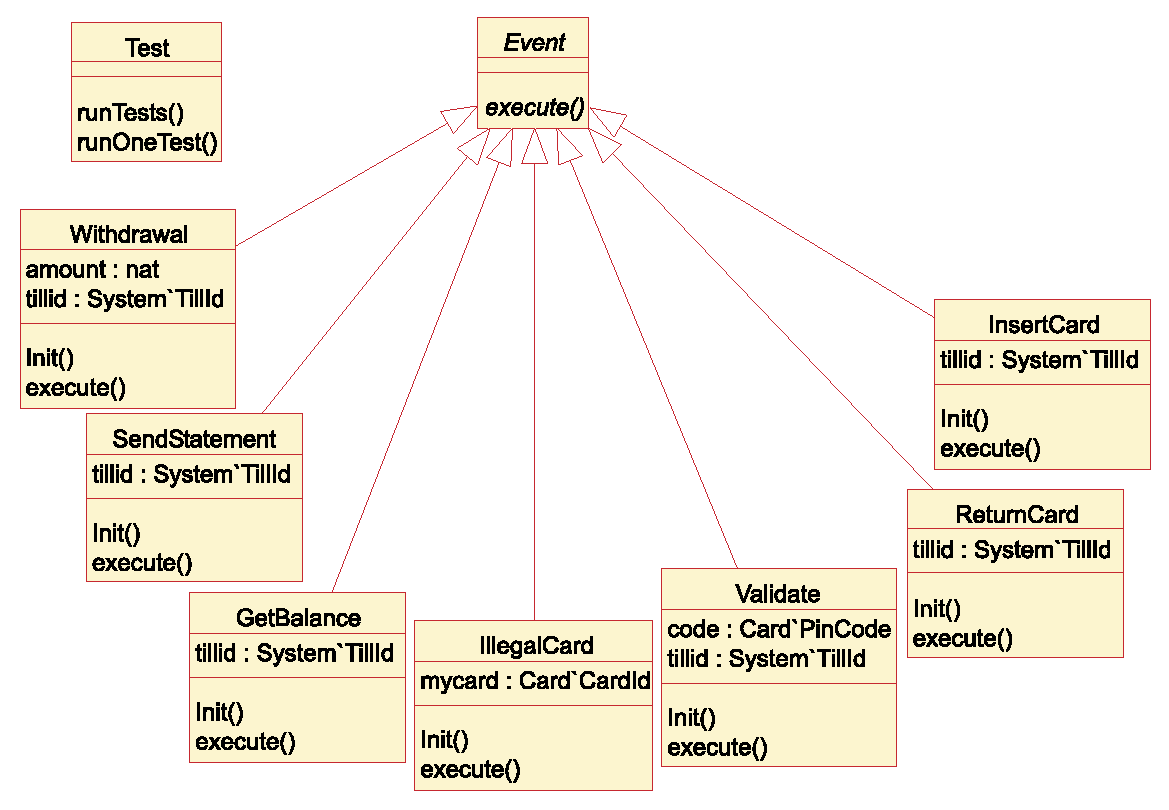
\includegraphics[width=.9\textwidth]{testing2}
\caption{An overview of the testing classes in UML.\label{fig:test}}
\end{center}
\end{figure}

\subsection{The Testing Classes}

In order to test the VDM++ model appropriately a small test class and
a series of small event classes are created (see
Figure~\ref{fig:test}). Each of these classes are structured as
subclasses of a general \texttt{\emph{Event}} class which has a
virtual operation called \texttt{\emph{execute}}. All these auxiliary
classes are listed below in pretty printed form without test coverage
because that is of no value for these classes. The actual testing is
carried out using two small batch-mode scripts. These scripts uses a
command-line version of \vdmtools\ with special options for the
collection of test coverage information.



\subsubsection{A Test Class}

The \texttt{\emph{Test}} class defines an environment for executing test cases. 
The class maintains a reference to an overall Cashpoint system, 
and it provides two operations, \texttt{\emph{runOneTest}} for execution 
of one test event, and \texttt{\emph{runTests}} for execution of a sequence 
of test events. Different kinds of test events can be executed. 
These are defined by the Event class hierarchy defined below.

The data types represent different kinds of categories of results 
which in this case are simply booleans, natural numbers, special quotes or nil.

\begin{VDMgray}
\textbf{class} \textit{Test}
\textbf{types}

 \textbf{public}
 \textit{TestResult} = \ensuremath{[}\textbf{bool} {\textbar} \textbf{nat} {\textbar} \texttt{<}PinOk\texttt{>} {\textbar} \texttt{<}PinNotOk\texttt{>} {\textbar} \texttt{<}Retained\texttt{>}\ensuremath{]}

\textbf{instance} \textbf{variables}

 \textit{system} : \textit{System} := \textbf{new} \textit{System}();

\textbf{operations}

 \textbf{public}
 \textit{runTests} : \textbf{seq} \textbf{of} \textit{Event} ==\texttt{>} \textbf{seq} \textbf{of} \textit{TestResult}
 \textit{runTests} (\textit{events}) ==
   (\textit{system} := \textit{system}.\textit{Init}();
    \textbf{return} \ensuremath{[}\textit{events}(\textit{i}).\textit{execute}(\textit{system}) {\textbar} \textit{i} \textbf{in set} \textbf{inds} \textit{events} \ensuremath{]});

 \textbf{public}
 \textit{runOneTest} : \textit{Event} ==\texttt{>} \textit{TestResult}
 \textit{runOneTest} (\textit{event}) ==
    \textbf{return} \textit{event}.\textit{execute}(\textit{system}.\textit{Init}());

\textbf{end} \textit{Test}
\end{VDMgray}

\newpage
\subsubsection{The Event Class}

The \texttt{\emph{Event}} class is the abstract super class of the class 
hierarchy of test events. Each class implementing this event 
class must define an \texttt{\emph{execute}} operation.

\begin{VDMgray}
\textbf{class} \textit{Event}

\textbf{operations}

 \textbf{public}
 \textit{execute} : \textit{System} ==\texttt{>} \textit{Test}\`{}\textit{TestResult}
 \textit{execute} (\textit{system}) ==
    \textbf{is} \textbf{subclass} \textbf{responsibility};

\textbf{end} \textit{Event}
\end{VDMgray}

\newpage

\subsubsection{The Withdrawal Testing Class}

The event \texttt{\emph{Withdraval}} corresponds to a client asking to withdraw 
money at one of the tills in this system.

\begin{VDMgray}
\textbf{class} \textit{Withdrawal} \textbf{is} \textbf{subclass} \textbf{of} \textit{Event}

\textbf{instance} \textbf{variables}

 \textit{tillid} : \textit{System}\`{}\textit{TillId};
 \textit{amount} : \textbf{nat};

\textbf{operations}

 \textbf{public}
 \textit{Init}: \textit{System}\`{}\textit{TillId} * \textbf{nat} ==\texttt{>} \textit{Withdrawal}
 \textit{Init}(\textit{t},\textit{a}) ==
   (\textit{tillid} := \textit{t};
    \textit{amount} := \textit{a};
    \textbf{return} \textbf{self});

 \textbf{public}
 \textit{execute}: \textit{System} ==\texttt{>} \textit{Test}\`{}\textit{TestResult}
 \textit{execute}(\textit{sys}) ==
   \textbf{let} \textit{till} = \textit{sys}.\textit{GetTill}(\textit{tillid})
   \textbf{in}
      \textbf{if} \textit{till}.\textit{CardValidated}()
      \textbf{then} \textit{till}.\textit{MakeWithdrawal}(\textit{amount})
      \textbf{else} \textbf{return} \textbf{false};

\textbf{end} \textit{Withdrawal}
\end{VDMgray}

\newpage

\subsubsection{The SendStatement Testing Class}

The event \texttt{\emph{SendStatement}} corresponds to a client asking for 
a statement to be sent by ordinary mail at one of the tills in 
this system.

\begin{VDMgray}
\textbf{class} \textit{SendStatement} \textbf{is} \textbf{subclass} \textbf{of} \textit{Event}

\textbf{instance} \textbf{variables}

 \textit{tillid} : \textit{System}\`{}\textit{TillId};

\textbf{operations}

 \textbf{public}
 \textit{Init}: \textit{System}\`{}\textit{TillId} ==\texttt{>} \textit{SendStatement}
 \textit{Init}(\textit{tid}) ==
   (\textit{tillid} := \textit{tid};
    \textbf{return} \textbf{self});

 \textbf{public}
 \textit{execute}: \textit{System} ==\texttt{>} \textit{Test}\`{}\textit{TestResult}
 \textit{execute}(\textit{sys}) ==
   \textbf{let} \textit{till} = \textit{sys}.\textit{GetTill}(\textit{tillid})
   \textbf{in}
      \textbf{if} \textit{till}.\textit{CardValidated}()
      \textbf{then} \textit{till}.\textit{RequestStatement}()
      \textbf{else} \textbf{return} \textbf{false};

\textbf{end} \textit{SendStatement}
\end{VDMgray}

\newpage
\subsubsection{The GetBalance Testing Class}

The event \texttt{\emph{GetBalance}} corresponds to a client asking for a 
balance at one of the tills in this system.

\begin{VDMgray}
\textbf{class} \textit{GetBalance} \textbf{is} \textbf{subclass} \textbf{of} \textit{Event}

\textbf{instance} \textbf{variables}

 \textit{tillid} : \textit{System}\`{}\textit{TillId};

\textbf{operations}

 \textbf{public}
 \textit{Init}: \textit{System}\`{}\textit{TillId} ==\texttt{>} \textit{GetBalance}
 \textit{Init}(\textit{tid}) ==
   (\textit{tillid} := \textit{tid};
    \textbf{return} \textbf{self});

 \textbf{public}
 \textit{execute}: \textit{System} ==\texttt{>} \textit{Test}\`{}\textit{TestResult}
 \textit{execute}(\textit{sys}) ==
   \textbf{let} \textit{till} = \textit{sys}.\textit{GetTill}(\textit{tillid})
   \textbf{in}
      \textbf{if} \textit{till}.\textit{CardValidated}()
      \textbf{then} \textit{till}.\textit{GetBalance}()
      \textbf{else} \textbf{return} \textbf{false};

\textbf{end} \textit{GetBalance}
\end{VDMgray}

\newpage
\subsubsection{The Validate Testing Class}

The event \texttt{\emph{Validate}} corresponds to a client asking for
the card which has been inserted at one of the tills in this system to
be validated.

\begin{VDMgray}
\textbf{class} \textit{Validate} \textbf{is} \textbf{subclass} \textbf{of} \textit{Event}

\textbf{instance} \textbf{variables}

 \textit{tillid} : \textit{System}\`{}\textit{TillId};
 \textit{code} : \textit{Card}\`{}\textit{PinCode};

\textbf{operations}

 \textbf{public}
 \textit{Init}: \textit{System}\`{}\textit{TillId} * \textit{Card}\`{}\textit{PinCode} ==\texttt{>} \textit{Validate}
 \textit{Init}(\textit{tid},\textit{pin}) ==
   (\textit{tillid} := \textit{tid};
    \textit{code} := \textit{pin};
    \textbf{return} \textbf{self});

 \textbf{public}
 \textit{execute}: \textit{System} ==\texttt{>} \textit{Test}\`{}\textit{TestResult}
 \textit{execute}(\textit{sys}) ==
   \textit{sys}.\textit{GetTill}(\textit{tillid}).\textit{Validate}(\textit{code});

\textbf{end} \textit{Validate}
\end{VDMgray}

\newpage
\subsubsection{The ReturnCard Testing Class}

The event \texttt{\emph{ReturnCard}} corresponds to a client asking to get 
the card out from one of the tills in this system.

\begin{VDMgray}
\textbf{class} \textit{ReturnCard} \textbf{is} \textbf{subclass} \textbf{of} \textit{Event}

\textbf{instance} \textbf{variables}

 \textit{tillid} : \textit{System}\`{}\textit{TillId};

\textbf{operations}

 \textbf{public}
 \textit{Init}: \textit{System}\`{}\textit{TillId} ==\texttt{>} \textit{ReturnCard}
 \textit{Init}(\textit{tid}) ==
   (\textit{tillid} := \textit{tid};
    \textbf{return} \textbf{self});

 \textbf{public}
 \textit{execute}: \textit{System} ==\texttt{>} \textit{Test}\`{}\textit{TestResult}
 \textit{execute}(\textit{sys}) ==
   (\textbf{let} \textit{till} = \textit{sys}.\textit{GetTill}(\textit{tillid})
    \textbf{in}
       \textbf{if} \textit{till}.\textit{CardInside}()
       \textbf{then} \textit{till}.\textit{ReturnCard}()
       \textbf{else} \textbf{return} \textbf{false};
    \textbf{return} \textbf{true});

\textbf{end} \textit{ReturnCard}
\end{VDMgray}

\newpage
\subsubsection{The InsertCard Testing Class}

The event \texttt{\emph{InsertCard}} corresponds to a client inserting a 
card at one of the tills in this system.

\begin{VDMgray}
\textbf{class} \textit{InsertCard} \textbf{is} \textbf{subclass} \textbf{of} \textit{Event}

\textbf{instance} \textbf{variables}

 \textit{tillid} : \textit{System}\`{}\textit{TillId};
 \textit{mycard} : \textit{Card};

\textbf{operations}

 \textbf{public}
 \textit{Init}: \textit{System}\`{}\textit{TillId} * \textit{Card} ==\texttt{>} \textit{InsertCard}
 \textit{Init}(\textit{tid},\textit{c}) ==
   (\textit{tillid} := \textit{tid};
    \textit{mycard} := \textit{c};
    \textbf{return} \textbf{self});

 \textbf{public}
 \textit{execute}: \textit{System} ==\texttt{>} \textit{Test}\`{}\textit{TestResult}
 \textit{execute}(\textit{sys}) ==
   (\textit{sys}.\textit{GetTill}(\textit{tillid}).\textit{InsertCard}(\textit{mycard});
    \textbf{return} \textbf{true});

\textbf{end} \textit{InsertCard}
\end{VDMgray}

\newpage
\section{Concurrent VDM++ Design}\label{app:Concur}


\begin{figure}[htbp]
\begin{center}
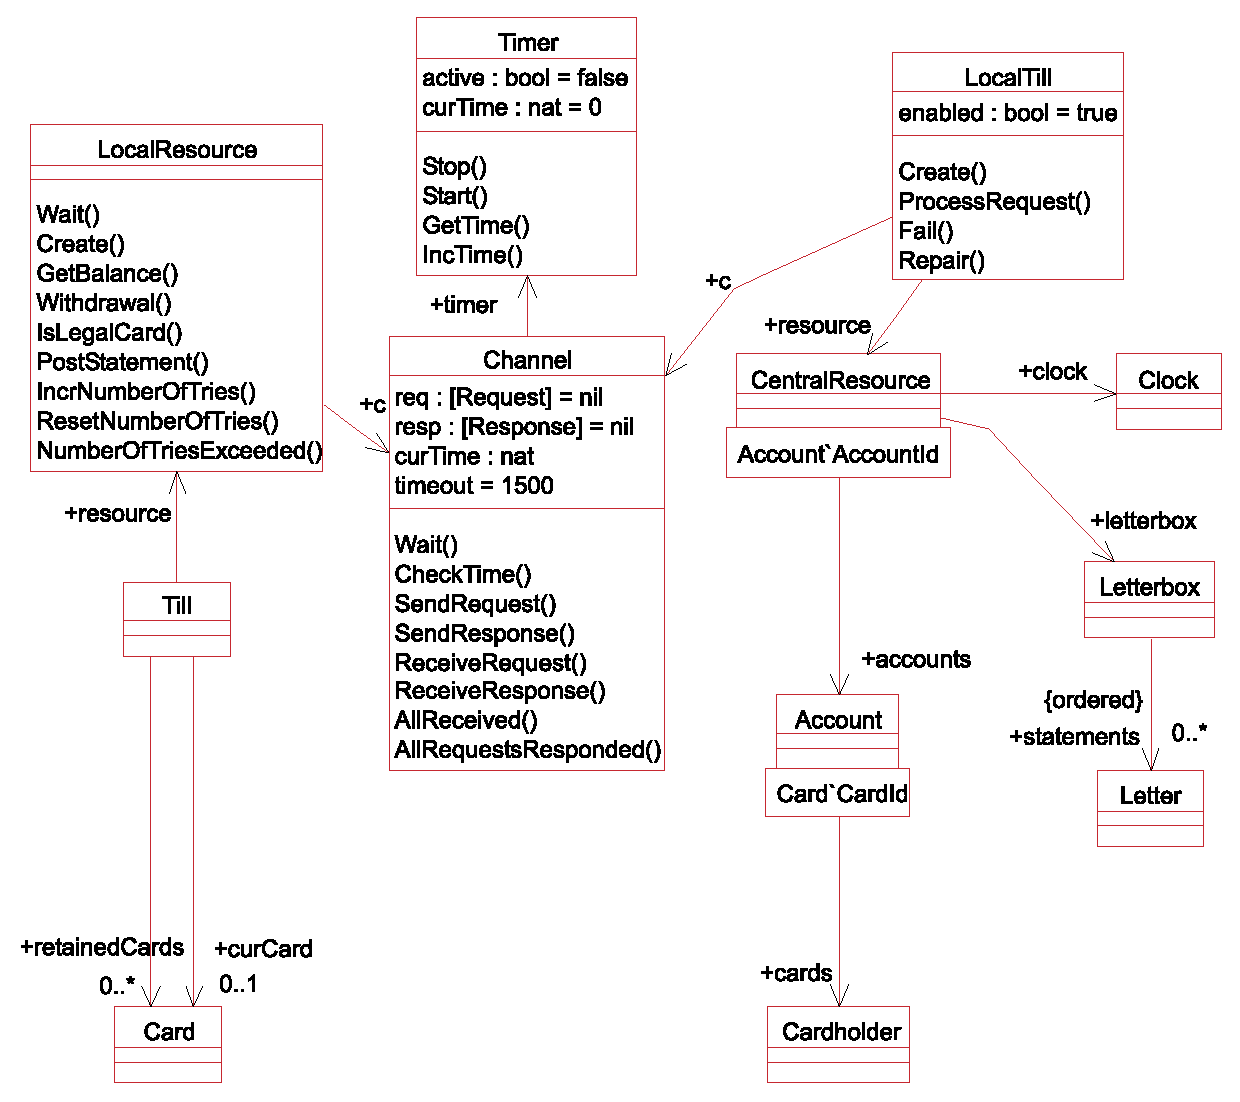
\includegraphics[width=.9\textwidth]{concurrent2}
\caption{UML Class Diagram for Concurrent model.\label{fig:UMLconcur}}
\end{center}
\end{figure}

In this Appendix we describe the enhanced VDM++ model which allows
modelling of communication failure. To achieve this four classes are
added: a \texttt{\emph{Channel}} for communication, and an associated
\texttt{\emph{Timer}} to allow timing out of communication; a
\texttt{\emph{LocalResource}}, which acts as an interface between a
\texttt{\emph{Till}} and a \texttt{\emph{Channel}}, providing a
virtually seamless replacement for the \texttt{\emph{Till}}'s
\texttt{\emph{CentralResource}} instance variable in the previous
model; and a \texttt{\emph{LocalTill}}, which acts as the interface
between a \texttt{\emph{Channel}} and a
\texttt{\emph{CentralResource}}.  These are shown in the UML class diagram
in Figure~\ref{fig:UMLconcur}. In this diagram, only those classes new to the model are shown
in detail; details  are not given for those classes reused from the
previous model.

\subsection{The Channel Class}


\begin{figure}[htbp]
\begin{center}
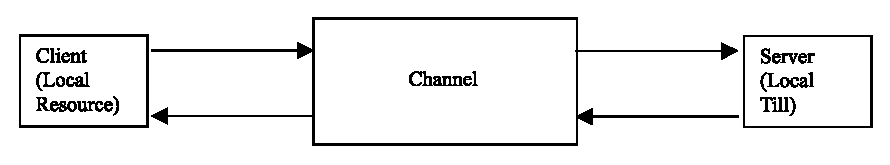
\includegraphics[width=5in]{channel2}
\caption{The client-server architecture.\label{fig:channel}}
\end{center}
\end{figure}

The \texttt{\emph{Channel}} class models communication between a
client (a \texttt{\emph{LocalResource}}) and a server (a
\texttt{\emph{LocalTill}}). It is a one place buffer which receives
requests from the client, which the server receives and processes. The
server generates a response to a given request which is sent to the
channel, and this response is then collected by the client. The
communication channel is considered to have failed if within some
predefined timeout interval starting from the moment a request was
received, response has not been received by the channel. This is
illustrated in Figure~\ref{fig:channel}.

\begin{VDMgray}
\textbf{class} \textit{Channel}
\end{VDMgray}


The channel has four instance variables: one each for storing 
incoming requests and responses, a reference to a \texttt{\emph{Timer}} object 
for timing out communication, and a counter (\texttt{\emph{curTime}}) which 
whenever a response is expected from the server, counts the time 
since the request was received from the client.

\begin{VDMgray}
\textbf{instance} \textbf{variables}
 \textit{req} : \ensuremath{[}\textit{Request}\ensuremath{]} := \textbf{nil};
 \textit{resp} :\ensuremath{[}\textit{Response}\ensuremath{]} := \textbf{nil};
 \textit{timer} : \textit{Timer} := \textbf{new} \textit{Timer}();
 \textit{curTime} : \textbf{nat};
\end{VDMgray}


The constant value timeout is an arbitrary constant used to model 
the amount of time we are prepared to wait before we conclude 
that the communication channel has failed. The actual value must
naturally be discussed with the bank.

\begin{VDMgray}
\textbf{values}
 \textit{timeout} = 1500;
\end{VDMgray}


A number of types are defined which are used to represent the 
values that are communicated through the channel.

\begin{VDMgray}
\textbf{types}
\end{VDMgray}


A request from a client consists of a command to the server, 
and any arguments relating to that command.

\begin{VDMgray}
 \textbf{public}
 \textit{Request} :: \textit{command} : \textit{Command}
            \textit{data} : \textbf{set} \textbf{of} \textit{ReqData};
\end{VDMgray}


A command is a quote value, corresponding to the possible operations 
that may be called in the  \texttt{\emph{CentralResource}}.

\begin{VDMgray}
 \textbf{public}
 \textit{Command} = \texttt{<}TriesExceeded\texttt{>} {\textbar} \texttt{<}ResetTries\texttt{>} {\textbar} \texttt{<}IncTries\texttt{>} {\textbar}
           \texttt{<}GetBalance\texttt{>} {\textbar} \texttt{<}Withdrawal\texttt{>} {\textbar} \texttt{<}PostStmt\texttt{>} {\textbar}
           \texttt{<}IsLegalCard\texttt{>};
\end{VDMgray}


An element of type \texttt{\emph{ReqData}} represents a possible argument to 
an operation in \texttt{\emph{CentralResource}}.

\begin{VDMgray}
 \textbf{public} \textit{ReqData} = \textit{CardId} {\textbar} \textit{AccountId} {\textbar} \textit{Amount};
 \textbf{public} \textit{CardId} :: \textit{val} : \textit{Card}\`{}\textit{CardId};
 \textbf{public} \textit{AccountId} :: \textit{val} : \textit{Account}\`{}\textit{AccountId};
 \textbf{public} \textit{Amount} :: \textit{val} : \textbf{nat};
\end{VDMgray}


A response consists of the command which is being responded to, and
the value computed by the corresponding operation in
\texttt{\emph{CentralResource}}.

\begin{VDMgray}
 \textbf{public}
 \textit{Response} :: \textit{command} : \textit{Command}
             \textit{data} : \textit{RespData};
 \textit{RespData} = \ensuremath{[}\textbf{nat}\ensuremath{]} {\textbar} \textbf{bool};
\end{VDMgray}

The operations available in this class represent the access operations 
on the buffer, together with a couple of auxilliary operations.

\begin{VDMgray}
\textbf{operations}
\end{VDMgray}

A client sends a request into the channel using \texttt{\emph{SendRequest}}. 
This takes a request and stores it in the appropriate instance 
variable, then resets the timer so that a timeout can be generated 
if necessary. As this is a one place buffer, we can only accept 
a request if there is not already one in the buffer (specified 
in the pre-condition).

\begin{VDMgray}
 \textbf{public}
 \textit{SendRequest} : \textit{Request} ==\texttt{>} ()
 \textit{SendRequest}(\textit{r}) ==
   (\textit{req} := \textit{r};
    \textit{timer}.\textit{Start}())
 \textbf{pre} \textit{req} = \textbf{nil};
\end{VDMgray}


The server removes requests from the buffer using \texttt{\emph{ReceiveRequest}}. 
This takes the request from the buffer and resets the corresponding 
instance variable to be \texttt{\textbf{nil}}.

\begin{VDMgray}
 \textbf{public}
 \textit{ReceiveRequest} : () ==\texttt{>} \textit{Request}
 \textit{ReceiveRequest}() ==
   \textbf{let} \textit{r} = \textit{req} \textbf{in}
      (\textit{req} := \textbf{nil};
       \textbf{return} \textit{r});
\end{VDMgray}


The server sends a response to the buffer using \texttt{\emph{SendResponse}}. 
The \texttt{\emph{resp}} instance variable is set to the value of the given response, 
and the timer is stopped as the response has been received. Again, 
the pre-condition specifies that a response can only be accepted 
if there is not already one waiting to be received by the client.

\begin{VDMgray}
 \textbf{public}
 \textit{SendResponse} : \textit{Response} ==\texttt{>} ()
 \textit{SendResponse}(\textit{r}) ==
   (\textit{resp} := \textit{r};
    \textit{timer}.\textit{Stop}())
 \textbf{pre} \textit{resp} = \textbf{nil};
\end{VDMgray}


The client receives a response using \texttt{\emph{ReceiveResponse}}. This delivers 
a response (if one has been received), or the \texttt{\textbf{nil}} value (representing 
a timeout). 

\begin{VDMgray}
 \textbf{public}
 \textit{ReceiveResponse} : () ==\texttt{>} \ensuremath{[}\textit{Response}\ensuremath{]}
 \textit{ReceiveResponse}() ==
   \textbf{let} \textit{r} = \textit{resp} \textbf{in}
     (\textit{resp} := \textbf{nil};
      \textbf{return} \textit{r});
\end{VDMgray}


The \texttt{\emph{Wait}} operation is used for synchronization. Its meaning will 
become clear when the synchronization constraints are described 
below.

\begin{VDMgray}
 \textbf{public}
 \textit{Wait}: () ==\texttt{>} ()
 \textit{Wait}() ==
   \textbf{skip};
\end{VDMgray}


The operation \texttt{\emph{CheckTime}} is executed periodically by the channel's 
thread, and is used to update the \texttt{\emph{curTime}} instance variable.

\begin{VDMgray}
 \textit{CheckTime}: () ==\texttt{>} ()
 \textit{CheckTime}() ==
   \textit{curTime} := \textit{timer}.\textit{GetTime}()
\end{VDMgray}


A function is defined which is used to simplify expressions in 
the synchronization constraints.The predicate \texttt{\emph{AllReceived}} takes 
the number of activations and completions of a send operation 
and the number of activations and completions of a receive operation, 
and returns true if and only if all of the send operations have 
completed, all of the receive operations have completed, and 
there corresponds a send operation for each receive operation.

\begin{VDMgray}
\textbf{functions}

 \textit{AllReceived} : \textbf{nat} * \textbf{nat} * \textbf{nat} * \textbf{nat} -\texttt{>} \textbf{bool}
 \textit{AllReceived}(\textit{act\_send}, \textit{fin\_send}, \textit{act\_rec}, \textit{fin\_rec}) ==
   \textit{act\_send} = \textit{fin\_send} \textbf{and}
   \textit{act\_rec} = \textit{fin\_rec} \textbf{and}
   \textit{act\_send} = \textit{act\_rec};
\end{VDMgray}


Since a \texttt{\emph{Channel}} object will be shared by both the client and 
the server, we specify permission predicates to ensure that the 
integrity of the object is preserved.

\begin{VDMgray}
\textbf{sync}
\end{VDMgray}


A \texttt{\emph{SendRequest}} can only be accepted if all previous
\texttt{\emph{SendRequest}}s have been received, all previous
\texttt{\emph{SendResponse}}s have been received, and the number of
requests equals the number of responses. This ensures that no requests
are accepted while a response to a previous request is being
processed.

\begin{VDMgray}
 \textbf{per} \textit{SendRequest} =\texttt{>}
   \textit{AllReceived}(\textbf{\#act}(\textit{SendRequest}), \textbf{\#fin}(\textit{SendRequest}),
        \textbf{\#act}(\textit{ReceiveRequest}), \textbf{\#fin}(\textit{ReceiveRequest})) \textbf{and}
   \textit{AllReceived}(\textbf{\#act}(\textit{SendResponse}), \textbf{\#fin}(\textit{SendResponse}),
        \textbf{\#act}(\textit{ReceiveResponse}), \textbf{\#fin}(\textit{ReceiveResponse})) \textbf{and}
   \textbf{\#act}(\textit{SendRequest}) = \textbf{\#fin}(\textit{ReceiveResponse});
\end{VDMgray}


The permission predicate on \texttt{\emph{SendResponse}} is similar to
\texttt{\emph{SendRequest}} except that the number of
\texttt{\emph{SendRequest}}s previously received must be exactly one
more than the number of \texttt{\emph{SendResponse}}s previously
received.

\begin{VDMgray}
 \textbf{per} \textit{SendResponse} =\texttt{>}
   \textit{AllReceived}(\textbf{\#act}(\textit{SendRequest}), \textbf{\#fin}(\textit{SendRequest}),
        \textbf{\#act}(\textit{ReceiveRequest}), \textbf{\#fin}(\textit{ReceiveRequest})) \textbf{and}
   \textit{AllReceived}(\textbf{\#act}(\textit{SendResponse}), \textbf{\#fin}(\textit{SendResponse}),
        \textbf{\#act}(\textit{ReceiveResponse}), \textbf{\#fin}(\textit{ReceiveResponse})) \textbf{and}
   \textbf{\#act}(\textit{SendRequest}) - \textbf{\#fin}(\textit{SendResponse}) = 1;
\end{VDMgray}


A request can only be received by the server if one has been placed in
the channel by the client. Until then a call to
\texttt{\emph{ReceiveRequest}} will block.

\begin{VDMgray}
 \textbf{per} \textit{ReceiveRequest} =\texttt{>} \textit{req} \texttt{<}\texttt{>} \textbf{nil};
\end{VDMgray}


The operation \texttt{\emph{Wait}} is used by a client to check
whether a response has been received for a request. Thus it will be
called by a client after sending a request. This call will block until
either a response has been received, or the current time exceeds the
timeout value.

\begin{VDMgray}
 \textbf{per} \textit{Wait} =\texttt{>} \textit{curTime} \texttt{>} \textit{timeout} \textbf{or} \textit{resp} \texttt{<}\texttt{>} \textbf{nil};
\end{VDMgray}


The only remaining part of the \texttt{\emph{Channel}} class is its
thread. This periodically calls \texttt{\emph{CheckTime}} to update
the time counter.

\begin{VDMgray}
\textbf{thread}
 \textbf{periodic}(1000)(\textit{CheckTime})

\textbf{end} \textit{Channel}
\end{VDMgray}


\subsection{The Class LocalResource}


A \texttt{\emph{LocalResource}} acts as a virtually seamless interface
for a till to a channel. Thus it provides the same calling interface
as a \texttt{\emph{CentralResource}}, except that its operations are
able to return the value \texttt{<}\texttt{\emph{Fail}}\texttt{>} to
represent a communication failure.

\begin{VDMgray}
\textbf{class} \textit{LocalResource}
\end{VDMgray}


A \texttt{\emph{LocalResource}} has only one instance variable: a reference to 
a \texttt{\emph{Channel}}.

\begin{VDMgray}
\textbf{instance} \textbf{variables}
 \textit{c} : \textit{Channel};

\textbf{operations}
\end{VDMgray}


The \texttt{\emph{Create}} operation is used to initialize the channel.

\begin{VDMgray}
 \textbf{public}
 \textit{Create} : \textit{Channel} ==\texttt{>} ()
 \textit{Create}(\textit{nc}) ==
   \textit{c} := \textit{nc};
\end{VDMgray}


The operation \texttt{\emph{GetBalance}} shadows the corresponding
operation in \texttt{\emph{CentralResource}}. The argument received by
the operation is converted into a value of type
\texttt{\emph{Channel\`{}ReqData}}, and then a request is
constructed. This is sent to the channel and then the
\texttt{\emph{Wait}} operation is called.

\begin{VDMgray}
 \textbf{public}
 \textit{GetBalance} : \textit{Account}\`{}\textit{AccountId} ==\texttt{>} \ensuremath{[}\textbf{nat}\ensuremath{]}{\textbar} \texttt{<}Fail\texttt{>}
 \textit{GetBalance}(\textit{accountId}) ==
   \textbf{let} \textit{req} = \textbf{mk\_}\textit{Channel}\`{}\textit{Request}(\texttt{<}GetBalance\texttt{>},
             \{\textbf{mk\_}\textit{Channel}\`{}\textit{AccountId}(\textit{accountId})\}) \textbf{in}
     (\textit{c}.\textit{SendRequest}(\textit{req});
      \textit{Wait}(\texttt{<}GetBalance\texttt{>}));
\end{VDMgray}


The \texttt{\emph{Wait}} operation waits for a particular response
from the channel.  If the response is \texttt{\textbf{nil}} or does
not match the expected result, a failure is signalled (corresponding
to a timeout in the \texttt{\emph{Channel}}).  Otherwise the data
value in the response is returned.

\begin{VDMgray}
 \textit{Wait} : \textit{Channel}\`{}\textit{Command} ==\texttt{>} \textit{Channel}\`{}\textit{RespData} {\textbar} \texttt{<}Fail\texttt{>}
 \textit{Wait}(\textit{comm}) ==
   (\textit{c}.\textit{Wait}();
    \textbf{let} \textit{resp} = \textit{c}.\textit{ReceiveResponse}() \textbf{in}
      \textbf{if} \textit{resp} = \textbf{nil}
      \textbf{then} \textbf{return} \texttt{<}Fail\texttt{>}
      \textbf{elseif} \textit{resp}.\textit{command} \texttt{<}\texttt{>} \textit{comm}
      \textbf{then} \textbf{return} \texttt{<}Fail\texttt{>}
      \textbf{else} \textbf{return} \textit{resp}.\textit{data});
\end{VDMgray}


The remaining operations follow the same basic approach as that 
of \texttt{\emph{GetBalance}}, and need no further explanation.

\begin{VDMgray}
 \textbf{public}
 \textit{Withdrawal} : \textit{Account}\`{}\textit{AccountId} * \textit{Card}\`{}\textit{CardId} * \textbf{nat} ==\texttt{>}
           \textbf{bool} {\textbar} \texttt{<}Fail\texttt{>}
 \textit{Withdrawal}(\textit{accountId},\textit{cardId},\textit{amount}) ==
   \textbf{let} \textit{req} = \textbf{mk\_}\textit{Channel}\`{}\textit{Request}(\texttt{<}Withdrawal\texttt{>},
             \{\textbf{mk\_}\textit{Channel}\`{}\textit{AccountId}(\textit{accountId}),
              \textbf{mk\_}\textit{Channel}\`{}\textit{CardId}(\textit{cardId}),
              \textbf{mk\_}\textit{Channel}\`{}\textit{Amount}(\textit{amount})\}) \textbf{in}
     (\textit{c}.\textit{SendRequest}(\textit{req});
      \textit{Wait}(\texttt{<}Withdrawal\texttt{>}));
\end{VDMgray}

\begin{VDMgray}
 \textbf{public}
 \textit{PostStatement} : \textit{Account}\`{}\textit{AccountId} * \textit{Card}\`{}\textit{CardId} ==\texttt{>}
                 \textbf{bool} {\textbar} \texttt{<}Fail\texttt{>}
 \textit{PostStatement}(\textit{accountId},\textit{cardId}) ==
   \textbf{let} \textit{req} = \textbf{mk\_}\textit{Channel}\`{}\textit{Request}(\texttt{<}PostStmt\texttt{>},
              \{\textbf{mk\_}\textit{Channel}\`{}\textit{AccountId}(\textit{accountId}),
               \textbf{mk\_}\textit{Channel}\`{}\textit{CardId}(\textit{cardId})\}) \textbf{in}
     (\textit{c}.\textit{SendRequest}(\textit{req});
      \textit{Wait}(\texttt{<}PostStmt\texttt{>}));
\end{VDMgray}

\begin{VDMgray}
 \textbf{public}
 \textit{IsLegalCard} : \textit{Account}\`{}\textit{AccountId} * \textit{Card}\`{}\textit{CardId} ==\texttt{>}
              \textbf{bool} {\textbar} \texttt{<}Fail\texttt{>}
 \textit{IsLegalCard}(\textit{accountId},\textit{cardId}) ==
   \textbf{let} \textit{req} = \textbf{mk\_}\textit{Channel}\`{}\textit{Request}(\texttt{<}IsLegalCard\texttt{>},
              \{\textbf{mk\_}\textit{Channel}\`{}\textit{AccountId}(\textit{accountId}),
               \textbf{mk\_}\textit{Channel}\`{}\textit{CardId}(\textit{cardId})\}) \textbf{in}
     (\textit{c}.\textit{SendRequest}(\textit{req});
      \textit{Wait}(\texttt{<}IsLegalCard\texttt{>}));
\end{VDMgray}

\begin{VDMgray}
 \textbf{public}
 \textit{NumberOfTriesExceeded} : \textit{Card}\`{}\textit{CardId} ==\texttt{>} \textbf{bool} {\textbar} \texttt{<}Fail\texttt{>}
 \textit{NumberOfTriesExceeded}(\textit{cardId}) ==
   \textbf{let} \textit{req} = \textbf{mk\_}\textit{Channel}\`{}\textit{Request}(\texttt{<}TriesExceeded\texttt{>},
              \{\textbf{mk\_}\textit{Channel}\`{}\textit{CardId}(\textit{cardId})\}) \textbf{in}
     (\textit{c}.\textit{SendRequest}(\textit{req});
      \textit{Wait}(\texttt{<}TriesExceeded\texttt{>}));
\end{VDMgray}

\begin{VDMgray}
 \textbf{public}
 \textit{ResetNumberOfTries} : \textit{Card}\`{}\textit{CardId} ==\texttt{>} \ensuremath{[}\texttt{<}Fail\texttt{>}\ensuremath{]}
 \textit{ResetNumberOfTries}(\textit{cardId}) ==
   \textbf{let} \textit{req} = \textbf{mk\_}\textit{Channel}\`{}\textit{Request}(\texttt{<}ResetTries\texttt{>},
              \{\textbf{mk\_}\textit{Channel}\`{}\textit{CardId}(\textit{cardId})\}) \textbf{in}
     (\textit{c}.\textit{SendRequest}(\textit{req});
      \textit{Wait}(\texttt{<}ResetTries\texttt{>}));
\end{VDMgray}

\begin{VDMgray}
 \textbf{public}
 \textit{IncrNumberOfTries} : \textit{Card}\`{}\textit{CardId} ==\texttt{>} \ensuremath{[}\texttt{<}Fail\texttt{>}\ensuremath{]}
 \textit{IncrNumberOfTries}(\textit{cardId}) ==
   \textbf{let} \textit{req} = \textbf{mk\_}\textit{Channel}\`{}\textit{Request}(\texttt{<}IncTries\texttt{>},
                        \{\textbf{mk\_}\textit{Channel}\`{}\textit{CardId}(\textit{cardId})\}) \textbf{in}
     (\textit{c}.\textit{SendRequest}(\textit{req});
      \textit{Wait}(\texttt{<}IncTries\texttt{>}));

\textbf{end} \textit{LocalResource}
\end{VDMgray}


\subsection{The Class LocalTill}

The class \texttt{\emph{LocalTill}} acts as an interface between a
\texttt{\emph{Channel}} and the \texttt{\emph{CentralResource}},
allowing the existing \texttt{\emph{CentralResource}} class to be used
without modification. At the heart of the class, requests are
repeatedly removed from the \texttt{\emph{Channel}}, processed, and
responses placed on the \texttt{\emph{Channel}}.

\begin{VDMgray}
\textbf{class} \textit{LocalTill}
\end{VDMgray}


Since it acts as an interface, the \texttt{\emph{LocalTill}} has
references to the two objects it mediates between: a
\texttt{\emph{Channel}} and the \texttt{\emph{CentralResource}}.  In
addition a boolean value is used to represent whether the
communication has failed or not (this is used for modelling purposes,
allowing us to test behaviour of the overall model in the presence of
failed communication).

\begin{VDMgray}
\textbf{instance} \textbf{variables}
 \textit{c}: \textit{Channel};
 \textit{resource} : \textit{CentralResource};
 \textit{enabled} : \textbf{bool} := \textbf{true};
\end{VDMgray}


The heart of this class is its thread, so we begin by describing 
it. The thread repeatedly receives requests from the \texttt{\emph{Channel}} 
and processes them, as long as enabled is true. Note that due 
to the permission predicates in \texttt{\emph{Channel}}, the call to \texttt{\emph{c.ReceiveRequest}} 
will block until a request has been sent by a till. Also, as 
well as the looping condition there is a second check of enabled 
in the body of the loop in case it has changed while the thread 
was waiting for a request.

\begin{VDMgray}
\textbf{thread}
 \textbf{while} \textit{enabled} \textbf{do}
 \textbf{let} \textit{req} = \textit{c}.\textit{ReceiveRequest}() \textbf{in}
   \textbf{if} \textit{enabled}
   \textbf{then} \textit{ProcessRequest}(\textit{req});
\end{VDMgray}


As can be seen from the thread, the main operation in this class is
\texttt{\emph{ProcessRequest}}. This takes a request, converts it into
a call to the \texttt{\emph{CentralResource}}, then converts the
result from \texttt{\emph{CentralResource}} into a response and sends
this to the \texttt{\emph{Channel}}. Of course the call to
\texttt{\emph{CentralResource}} will depend upon the kind of request
made, so a case statement is used to distinguish these requests.

\begin{VDMgray}
\textbf{operations}

 \textit{ProcessRequest} : \textit{Channel}\`{}\textit{Request} ==\texttt{>} ()
 \textit{ProcessRequest}(\textit{req}) ==
   (\textbf{dcl} \textit{respdata} : \textit{Channel}\`{}\textit{RespData};
    \textbf{cases} \textit{req}:
      \textbf{mk\_}\textit{Channel}\`{}\textit{Request}(
         \texttt{<}Withdrawal\texttt{>}, \{\textbf{mk\_}\textit{Channel}\`{}\textit{AccountId}(\textit{accId}),
                        \textbf{mk\_}\textit{Channel}\`{}\textit{CardId}(\textit{cardId}),
                        \textbf{mk\_}\textit{Channel}\`{}\textit{Amount}(\textit{amt})\})
       -\texttt{>} \textit{respdata} := \textit{resource}.
                              \textit{Withdrawal}(\textit{accId}, \textit{cardId}, \textit{amt}),
      \textbf{mk\_}\textit{Channel}\`{}\textit{Request}(
         \texttt{<}PostStmt\texttt{>}, \{\textbf{mk\_}\textit{Channel}\`{}\textit{AccountId}(\textit{accId}),
                      \textbf{mk\_}\textit{Channel}\`{}\textit{CardId}(\textit{cardId})\})
       -\texttt{>} \textit{respdata} := \textit{resource}.\textit{PostStatement}(\textit{accId}, \textit{cardId}),
      \textbf{mk\_}\textit{Channel}\`{}\textit{Request}(
         \texttt{<}IsLegalCard\texttt{>}, \{\textbf{mk\_}\textit{Channel}\`{}\textit{AccountId}(\textit{accId}),
                         \textbf{mk\_}\textit{Channel}\`{}\textit{CardId}(\textit{cardId})\})
       -\texttt{>} \textit{respdata} := \textit{resource}.\textit{IsLegalCard}(\textit{accId}, \textit{cardId}),
      \textbf{mk\_}\textit{Channel}\`{}\textit{Request}(
         \texttt{<}GetBalance\texttt{>}, \{\textbf{mk\_}\textit{Channel}\`{}\textit{AccountId}(\textit{accId})\})
       -\texttt{>} \textit{respdata} := \textit{resource}.\textit{GetBalance}(\textit{accId}),
      \textbf{mk\_}\textit{Channel}\`{}\textit{Request}(
         \texttt{<}TriesExceeded\texttt{>}, \{\textbf{mk\_}\textit{Channel}\`{}\textit{CardId}(\textit{cardId})\})
       -\texttt{>} \textit{respdata} := \textit{resource}.\textit{NumberOfTriesExceeded}(\textit{cardId}),
      \textbf{mk\_}\textit{Channel}\`{}\textit{Request}(
         \texttt{<}ResetTries\texttt{>}, \{\textbf{mk\_}\textit{Channel}\`{}\textit{CardId}(\textit{cardId})\})
       -\texttt{>} (\textit{resource}.\textit{ResetNumberOfTries}(\textit{cardId});
           \textit{respdata} := \textbf{nil}),
      \textbf{mk\_}\textit{Channel}\`{}\textit{Request}(
         \texttt{<}IncTries\texttt{>}, \{\textbf{mk\_}\textit{Channel}\`{}\textit{CardId}(\textit{cardId})\})
       -\texttt{>} (\textit{resource}.\textit{IncrNumberOfTries}(\textit{cardId});
           \textit{respdata} := \textbf{nil})
   \textbf{end};
   \textit{c}.\textit{SendResponse}
             (\textbf{mk\_}\textit{Channel}\`{}\textit{Response}(\textit{req}.\textit{command}, \textit{respdata})));
\end{VDMgray}


Finally we have a few minor operations. \texttt{\emph{Create}} is used
to initialize the \texttt{\emph{Channel}} and the
\texttt{\emph{CentralResource}}.

\begin{VDMgray}
 \textbf{public}
 \textit{Create} : \textit{Channel} * \textit{CentralResource} ==\texttt{>} ()
 \textit{Create}(\textit{nc}, \textit{nr}) ==
   (\textit{c} := \textit{nc};
    \textit{resource} := \textit{nr});
\end{VDMgray}


\texttt{\emph{Fail}} is used to set the enabled flag to false, when we wish to 
analyse the behaviour of failed communication.

\begin{VDMgray}
 \textit{Fail} : () ==\texttt{>} ()
 \textit{Fail}() ==
   \textit{enabled} := \textbf{false};
\end{VDMgray}


\texttt{\emph{Repair}} is used if we wish to reset the communication
following a failure. Note that a fresh \texttt{\emph{Channel}} is used
as this gives consistent history counters.

\begin{VDMgray}
 \textit{Repair} : \textit{Channel} ==\texttt{>} ()
 \textit{Repair}(\textit{nc}) ==
   (\textit{c} := \textit{nc};
    \textit{enabled} := \textbf{true});

\textbf{end} \textit{LocalTill}
\end{VDMgray}


\subsection{The Class Till}

The \texttt{\emph{Till}} class is virtually identical to the one
presented in Appendix B except that some of the operations have been
modified to be able to deliver the value
\texttt{<}\texttt{\emph{Fail}}\texttt{>} to represent failed
communication with the \texttt{\emph{CentralResource}}. Also, the
resource instance variable is now a reference to a
\texttt{\emph{LocalResource}}, though since
\texttt{\emph{LocalResource}} and \texttt{\emph{CentralResource}} have
an identical calling interface, this change is minimal. The remaining
changes are self-explanatory, so in the sequel we merely present the
class, with any changes from the previous version indicated by
underlining.

\begin{VDMgray}
\textbf{class} \textit{Till}

\textbf{instance} \textbf{variables}
 \textit{curCard} : \ensuremath{[}\textit{Card}\ensuremath{]} := \textbf{nil};
 \textit{cardOk} : \textbf{bool} := \textbf{false};
 \textit{retainedCards} : \textbf{set} \textbf{of} \textit{Card} := \{\};
 \textit{resource} : {\underline{LocalResource}}{\underline{;}}
 \textbf{inv} \textit{curCard} = \textbf{nil} =\texttt{>} \textbf{not} \textit{cardOk};

\textbf{operations}
 \textbf{public}
 \textit{Create}: \textit{LocalResource} ==\texttt{>} \textit{Till}
 \textit{Create}(\textit{res}) ==
   (\textit{resource} := \textit{res};
    \textbf{return} \textbf{self});

 \textbf{public}
 \textit{InsertCard} : \textit{Card} ==\texttt{>} ()
 \textit{InsertCard}(\textit{c}) ==
   \textit{curCard} := \textit{c}
 \textbf{pre} \textbf{not} \textit{CardInside}();
\end{VDMgray}

\begin{VDMgray}
 \textbf{public}
 \textit{Validate} : \textit{Card}\`{}\textit{PinCode} ==\texttt{>} \texttt{<}PinOk\texttt{>} {\textbar} \texttt{<}PinNotOk\texttt{>} {\textbar} \texttt{<}Retained\texttt{>} {\textbar}
                             \texttt{<}Fail\texttt{>}
 \textit{Validate}(\textit{pin}) ==
   \textbf{let} \textit{cardId} = \textit{curCard}.\textit{GetCardId}(),
       \textit{codeOk} = \textit{curCard}.\textit{GetCode}() = \textit{Encode}(\textit{pin}),
       \textit{cardLegal} = \textit{IsLegalCard}()
   \textbf{in} \textbf{{\underline{if}}} \textit{{\underline{cardLegal}}} {\underline{= \texttt{<}Fail\texttt{>}}}
      \textbf{{\underline{then}}} \textbf{{\underline{return}}} {\underline{\texttt{<}Fail\texttt{>}}}
      \textbf{{\underline{else}}}
         (\textit{cardOk} := \textit{codeOk} \textbf{and} \textit{cardLegal};
          \textbf{if} \textbf{not} \textit{cardLegal}
          \textbf{then} (\textit{retainedCards} := \textit{retainedCards} \textbf{union}
	                             \{\textit{curCard}\};
          \textit{curCard} := \textbf{nil};
          \textbf{return} \texttt{<}Retained\texttt{>})
      \textbf{elseif} \textit{codeOk}
      \textbf{{\underline{then}}} \textbf{{\underline{if}}} \textit{{\underline{resource}}}{\underline{.}}\textit{{\underline{ResetNumberOfTries}}}{\underline{(}}\textit{{\underline{cardId}}}{\underline{) 
= \texttt{<}Fail\texttt{>}}}
              \textbf{{\underline{then}}} \textbf{{\underline{return}}} {\underline{\texttt{<}Fail\texttt{>}}}
              \textbf{{\underline{else}}} \textbf{{\underline{return}}} {\underline{\texttt{<}PinOk\texttt{>}}}
      \textbf{{\underline{else}}}
         {\underline{(}}\textbf{{\underline{let}}} \textit{{\underline{incTries}}} {\underline{=}} \textit{{\underline{resource}}}{\underline{.}}\textit{{\underline{IncrNumberOfTries}}}{\underline{(}}\textit{{\underline{cardId}}}{\underline{),}}
             \textit{{\underline{numTriesExceeded}}} {\underline{=}}
                    \textit{{\underline{resource}}}{\underline{.}}\textit{{\underline{NumberOfTriesExceeded}}}{\underline{(}}\textit{{\underline{cardId}}}{\underline{)}} \textbf{{\underline{in}}}
            \textbf{{\underline{if}}} {\underline{\texttt{<}Fail\texttt{>}}} \textbf{{\underline{in set}}} {\underline{\{}}\textit{{\underline{incTries}}}{\underline{,}} \textit{{\underline{numTriesExceeded}}}{\underline{\}}}
            \textbf{{\underline{then}}} \textbf{{\underline{return}}} {\underline{\texttt{<}Fail\texttt{>}}}
            \textbf{{\underline{elseif}}} \textit{{\underline{numTriesExceeded}}} \textbf{then}
              (\textit{retainedCards} := \textit{retainedCards} \textbf{union}
                                \{\textit{curCard}\};
               \textit{cardOk} := \textbf{false};
               \textit{curCard} := \textbf{nil};
               \textbf{{\underline{return}}} {\underline{\texttt{<}Retained\texttt{>})}}
            \textbf{{\underline{else}}} \textbf{{\underline{return}}} {\underline{\texttt{<}PinNotOk\texttt{>}}}
            )
       )
 \textbf{pre} \textit{CardInside}() \textbf{and} \textbf{not} \textit{cardOk};
\end{VDMgray}

\begin{VDMgray}
 \textbf{public}
 \textit{ReturnCard} : () ==\texttt{>} ()
 \textit{ReturnCard}() ==
   (\textit{cardOk} := \textbf{false};
    \textit{curCard}:= \textbf{nil})
  \textbf{pre} \textit{CardInside}();

 \textbf{public}
 \textit{GetBalance} : () ==\texttt{>} \ensuremath{[}\textbf{nat}\ensuremath{]}{\underline{{\textbar}\texttt{<}Fail\texttt{>}}}
 \textit{GetBalance}() ==
   \textit{resource}.\textit{GetBalance}(\textit{curCard}.\textit{GetAccountId}())
 \textbf{pre} \textit{CardValidated}();
\end{VDMgray}

\begin{VDMgray}
 \textbf{public}
 \textit{MakeWithdrawal} : \textbf{nat} ==\texttt{>} \textbf{bool} {\underline{{\textbar} \texttt{<}Fail\texttt{>}}}
 \textit{MakeWithdrawal}(\textit{amount}) ==
   \textit{resource}.\textit{Withdrawal}
     (\textit{curCard}.\textit{GetAccountId}(),\textit{curCard}.\textit{GetCardId}(),\textit{amount})
 \textbf{pre} \textit{CardValidated}();

 \textbf{public}
 \textit{RequestStatement} : () ==\texttt{>} \textbf{bool} {\underline{{\textbar} \texttt{<}Fail\texttt{>}}}
 \textit{RequestStatement}() ==
   \textit{resource}.\textit{PostStatement}(\textit{curCard}.\textit{GetAccountId}(),
                                      \textit{curCard}.\textit{GetCardId}())
 \textbf{pre} \textit{CardValidated}();
\end{VDMgray}


The \texttt{\emph{IsLegalCard}} operation below is only used internally to validate 
a card.

\begin{VDMgray}
 \textbf{public}
 \textit{IsLegalCard} : () ==\texttt{>} \textbf{bool} {\underline{{\textbar} \texttt{<}Fail\texttt{>}}}
 \textit{IsLegalCard}() ==
   \textbf{return} \textit{resource}.\textit{IsLegalCard}(\textit{curCard}.\textit{GetAccountId}(),
                               \textit{curCard}.\textit{GetCardId}())
 \textbf{pre} \textit{CardInside}();

 \textbf{public}
 \textit{CardValidated}: () ==\texttt{>} \textbf{bool}
 \textit{CardValidated}() ==
   \textbf{return} \textit{curCard} \texttt{<}\texttt{>} \textbf{nil} \textbf{and} \textit{cardOk};

 \textbf{public}
 \textit{CardInside}: () ==\texttt{>} \textbf{bool}
 \textit{CardInside}() ==
   \textbf{return} \textit{curCard} \texttt{<}\texttt{>} \textbf{nil};

\textbf{functions}


 \textit{Encode}: \textit{Card}\`{}\textit{PinCode} +\texttt{>} \textit{Card}\`{}\textit{Code}
 \textit{Encode}(\textit{pin}) ==
   \textit{pin};
   -- The actual encoding procedure has not yet been chosen

\textbf{end} \textit{Till}
\end{VDMgray}

\subsection{The Timer Class}

The \texttt{\emph{Timer}} class is a straightforward periodic timer
which increments its clock in its own thread. It provides operations
for starting, and stopping timing, and reading the current time.

\begin{VDMgray}
\textbf{class} \textit{Timer}
\end{VDMgray}


The Timer has two instance variables for the current time and a flag
indicating whether the \texttt{\emph{Timer}} is active or not (the
current time is only incremented if the \texttt{\emph{Timer}} is
active).

\begin{VDMgray}
\textbf{instance} \textbf{variables}
 \textit{curTime} : \textbf{nat} := 0;
 \textit{active} : \textbf{bool} := \textbf{false};
\end{VDMgray}


The Timer provides straightforward operations which need no further 
explanation.

\begin{VDMgray}
\textbf{operations}
 \textbf{public}
 \textit{Start} : () ==\texttt{>} ()
 \textit{Start}() ==
   (\textit{active} := \textbf{true};
    \textit{curTime} := 0);

 \textbf{public}
 \textit{Stop} : () ==\texttt{>} ()
 \textit{Stop}() ==
   \textit{active} := \textbf{false};

 \textbf{public}
 \textit{GetTime} : () ==\texttt{>} \textbf{nat}
 \textit{GetTime}() ==
   \textbf{return} \textit{curTime};

 \textit{IncTime}: () ==\texttt{>} ()
 \textit{IncTime}() ==
   \textbf{if} \textit{active}
   \textbf{then} \textit{curTime} := \textit{curTime} + 100;
\end{VDMgray}


The Timer's thread ensures that the current time is incremented. 
We take one time unit for our Timer to correspond to 10 system 
time units.

\begin{VDMgray}
\textbf{thread}
 \textbf{periodic}(1000)(\textit{IncTime})

\textbf{end} \textit{Timer
}
\end{VDMgray}

\newpage
\subsection{Automatic Code Generation}

Having constructed a distributed VDM++ model, using \vdmtools\  
Java code was automatically generated. This code includes generation 
of permission predicates and thread definitions. Thus when combined 
with driver code, multithreaded code could be executed in which 
access to shared objects is guarded by permission predicates. The
automatically generated code is combined with the GUI shown in
Figure~\ref{fig:ppscreen} on page~\pageref{fig:ppscreen}. 

Below some sample output of an execution in batch mode is shown.
In this sample, four different tills are shown, with interaction 
at each till. At till 1, following insertion of the card and 
validation of the pin code, the communication channel fails. 
At tills 2, 3 and 4, three different cards on the same account 
are used so correct update of the shared balance can be observed.
Note that different executions of this Java program will result in
different traces because of the inherit non-determinism in the
concurrent VDM++ model.

\begin{alltt}
paulm@merry java mymain
Till 1: Validate Successful
Till 2: Validate Successful
Till 3: Validate Successful
Till 4: Validate Successful
Till 3: Balance is 3000
Till 4: Balance is 3000
Till 1: LocalTill Fail
Till 4: Withdrawal (100) Successful
Till 4: Balance is 2900
Till 2: Balance is 2900
Till 2: Withdrawal (100) Successful
Till 2: Balance is 2800
Till 3: Withdrawal (100) Successful
Till 3: Balance is 2700
Till 4: Card Returned
Till 2: Card Returned
Till 3: Card Returned
Till 1: Balance Failed
Till 1: Withdrawal (100) Failed
Till 1: Balance Failed
Till 1: Card Returned
\end{alltt}




\end{document}
